% Лабораторная работа по АСиСу № 4
% Михедов Константин Константинович

% Тип документа: статья, на бумаге А4
\documentclass[a4paper]{article}

% Подключение сторонних tex файлов 
\usepackage{import}


% Основные данные - ВУЗ, факультет, город...
\import{./../../stuff/tex}{config.tex}

% Подключение необходимых зависимостей
\import{./../../stuff/tex/settings}{packages.tex}
% Настройка подключенных пакетов
\import{./../../stuff/tex/settings}{preferences.tex}


% Шаблон титульной страницы 
\import{./../../stuff/tex/templates}{title.tex}
% Упрощенный блок "выполнил"
\import{./../../stuff/tex/templates}{sign1.tex}
% Макрос для содержания
\import{./../../stuff/tex/templates}{toc.tex}

% Определяем название документа
\title{
  Лабораторная работа №4 по курсу \\
  <<Проектный семинар>>  
}
% Отключаем отображение правительства
\renewcommand{\government}{}
% Отключаем сокращенное нзавание университета
\renewcommand{\subuniversity}{}
% Указываем преподавателя
\renewcommand{\shortteachername}{Минченков В.О.}


% Путь до внешних изображений
\graphicspath{ {./figures/}}


% Основной текст работы
\begin{document}
  \templatedtitlepage
  
  \toc

  \section{Ход работы}

  \subsection{Подготовка}

  \subsubsection{Настройка сети}

  Для выполнения данной работы потребуется две виртуальные машины, имеющие сетевой доступ
  друг к другу. Создадим \textit{NAT} сеть, которая позволит это сделать:

  \begin{figure}[H]
    \centering
    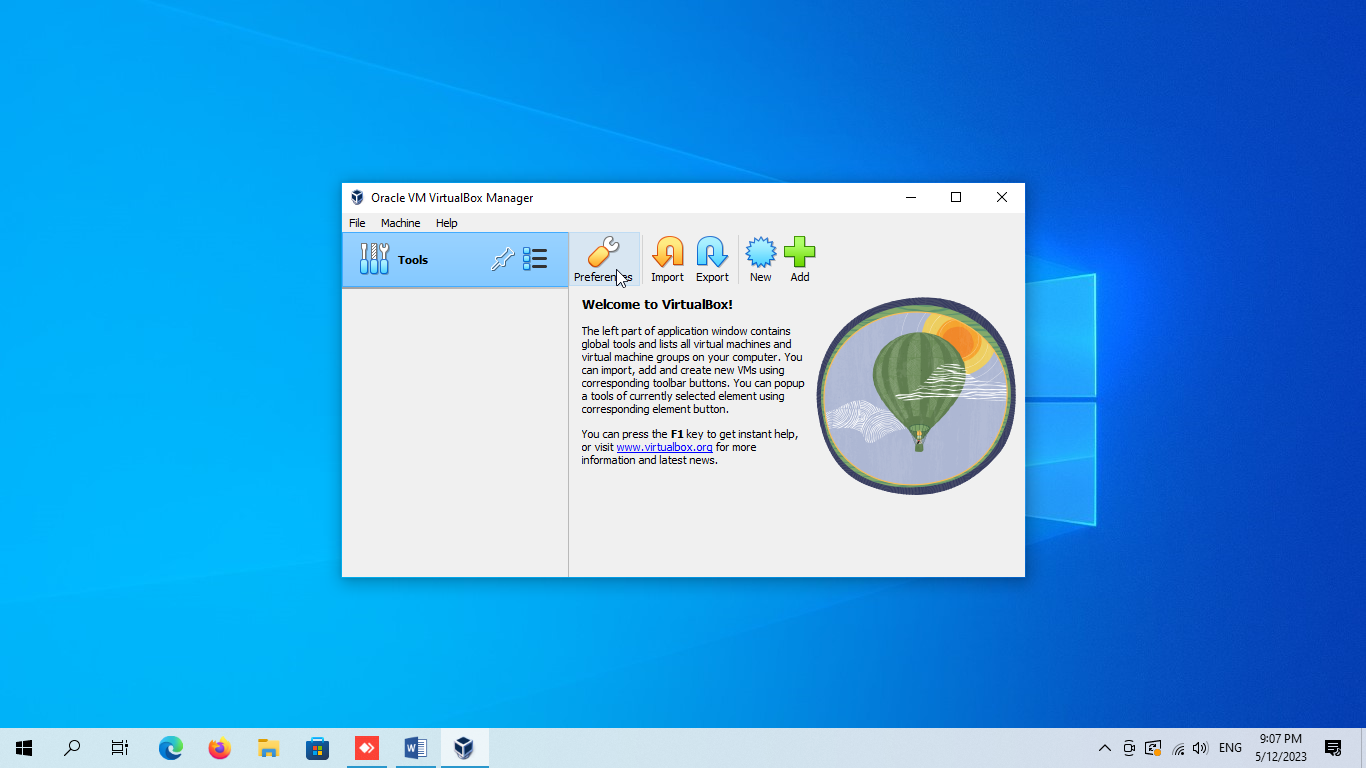
\includegraphics[width=0.85\textwidth]{04_0000}
    \label{img:0}
    \caption{Запускаем \textit{VirtualBox}}
  \end{figure}

  \begin{figure}[H]
    \centering
    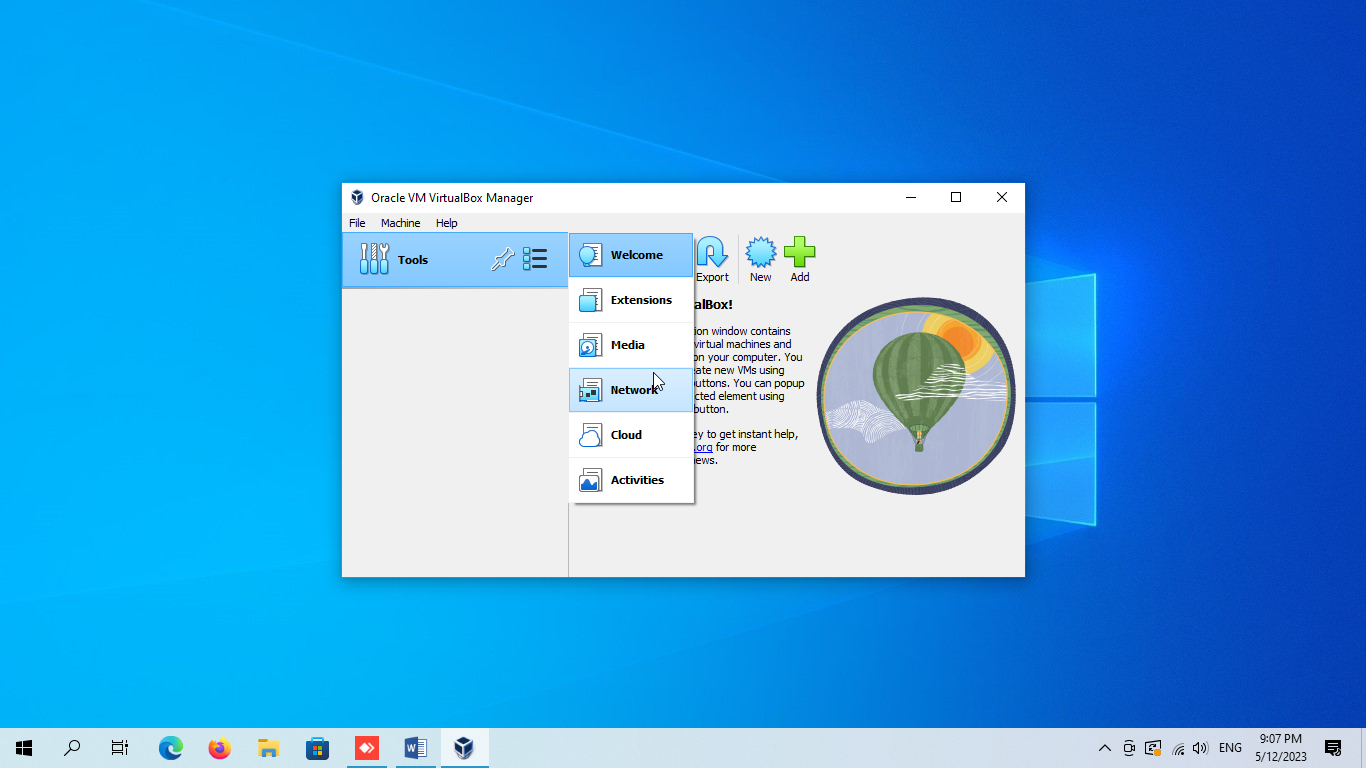
\includegraphics[width=0.85\textwidth]{04_0001}
    \label{img:1}
    \caption{Открываем настройки сети}
  \end{figure}

  \begin{figure}[H]
    \centering
    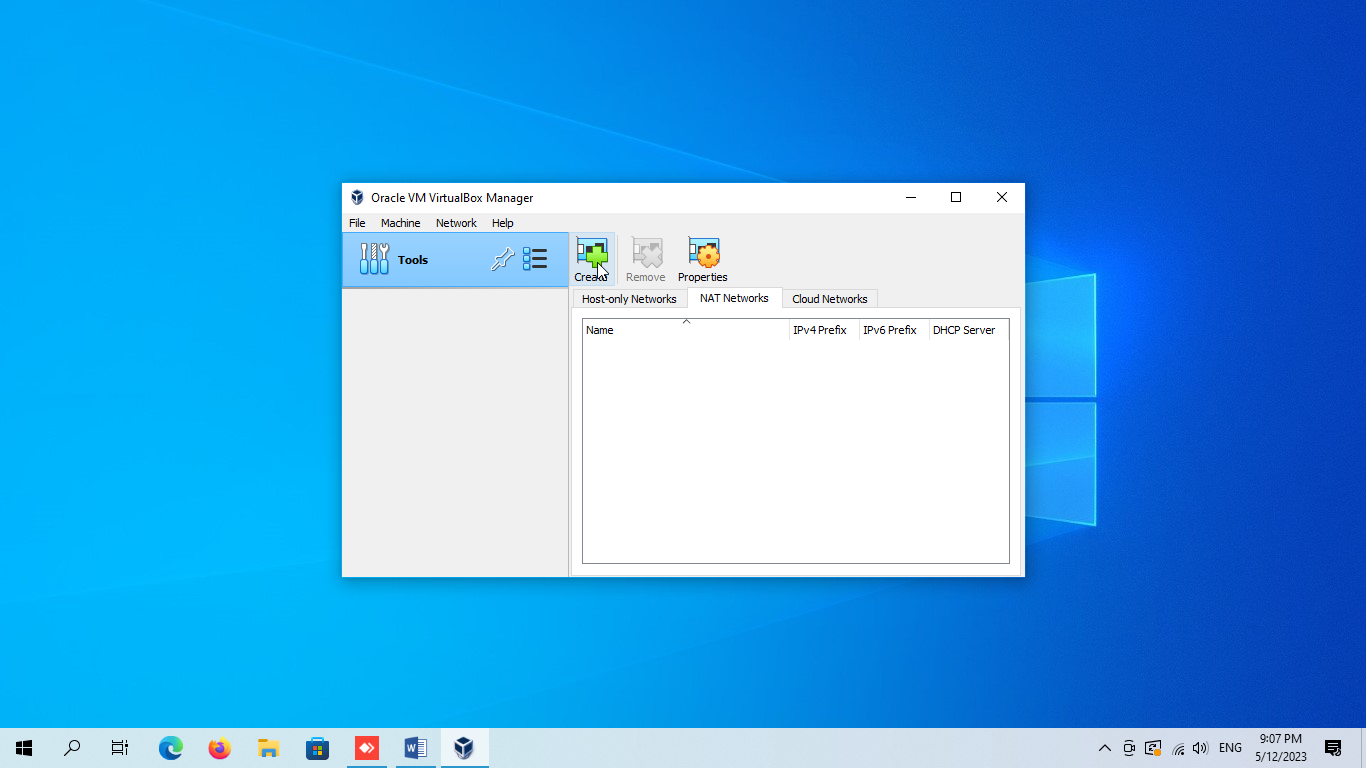
\includegraphics[width=0.85\textwidth]{04_0002}
    \label{img:2}
    \caption{Добавляем новую \textit{NAT} сеть}
  \end{figure}

  \begin{figure}[H]
    \centering
    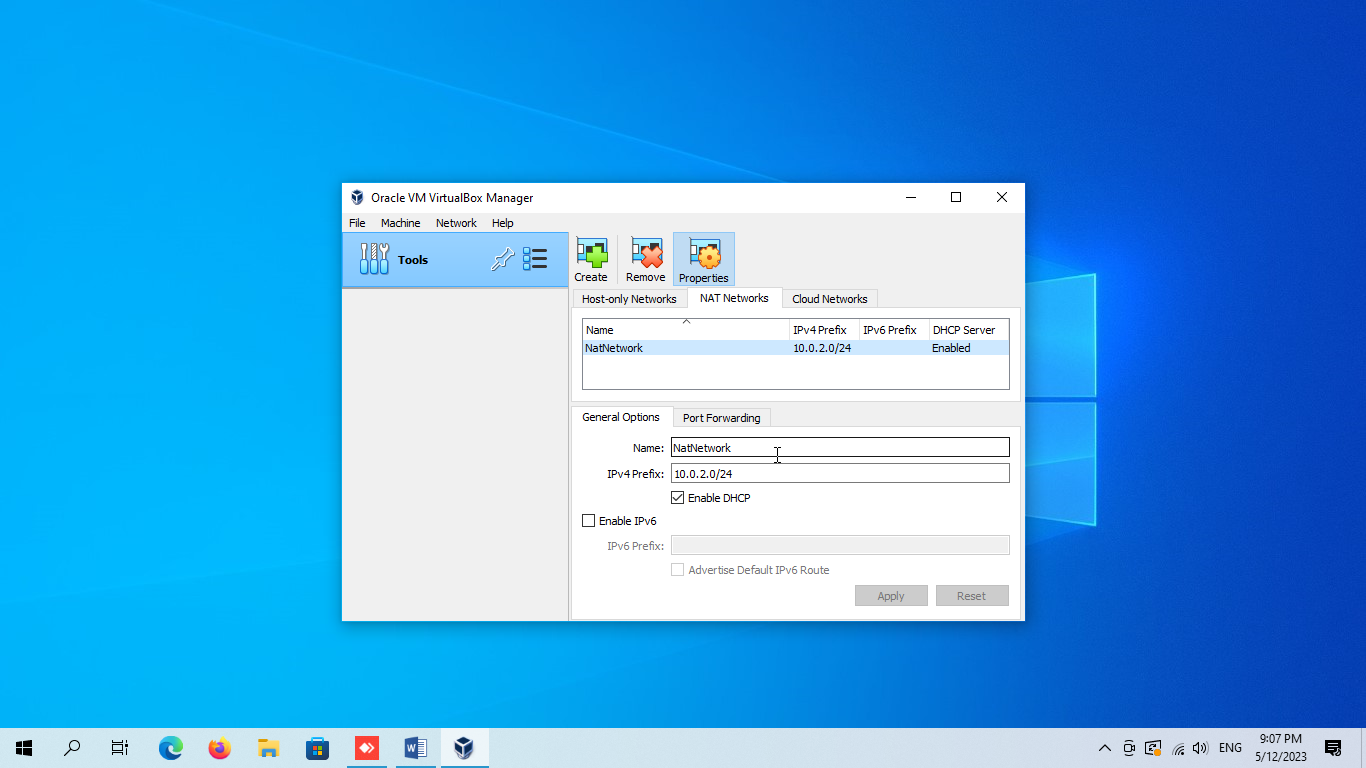
\includegraphics[width=0.85\textwidth]{04_0003}
    \label{img:3}
    \caption{Указываем параметры сети}
  \end{figure}

  Программа автоматически сгенерировала случайный адрес для созданной сети - 10.0.2.0/24.
  Оставим его как есть, а также включим встроенный \textit{DHCP} сервер, чтобы не заниматься
  ручной настройкой \textit{IP} адресов.

  \subsubsection{Создание виртуальных машин}

  Потребуются атакуемая и атакующая машина. В качестве атакуемой будем использовать
  специально подготовленный образ \textit{Metasploitable}, созданный специально для
  тестирования на нем уязвимостей:

  \begin{figure}[H]
    \centering
    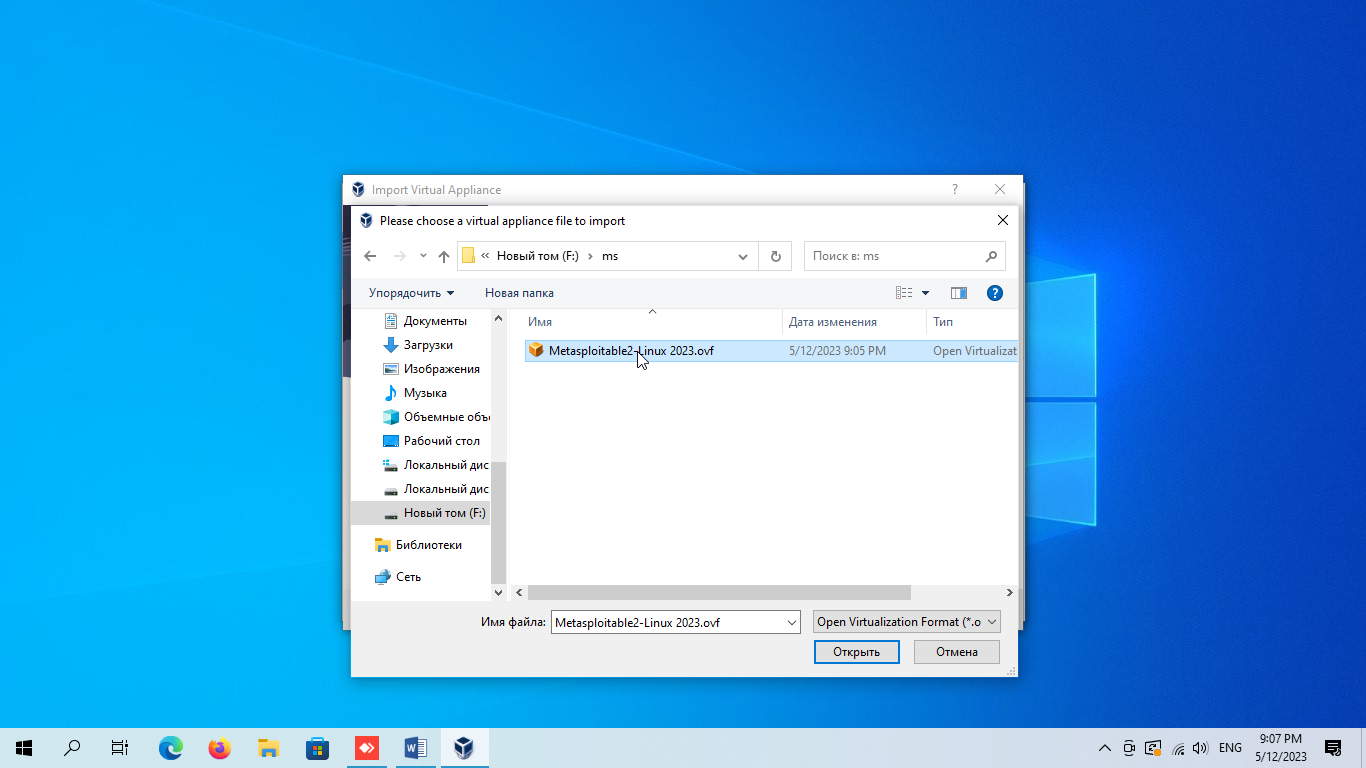
\includegraphics[width=0.85\textwidth]{04_0004}
    \label{img:4}
    \caption{Импортируем образ атакуемой машины}
  \end{figure}

  \begin{figure}[H]
    \centering
    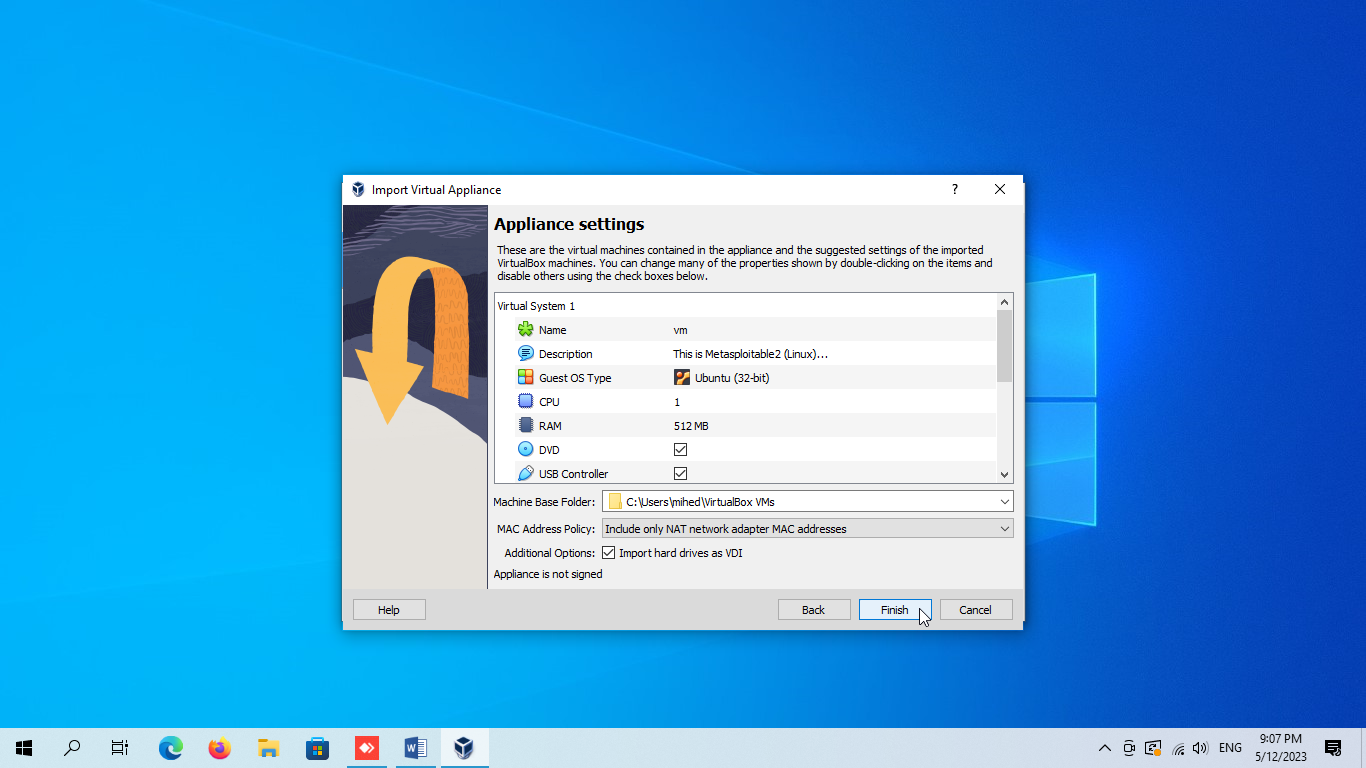
\includegraphics[width=0.85\textwidth]{04_0005}
    \label{img:5}
    \caption{Оставляем предложенные настройки как есть}
  \end{figure}

  Далее необходимо подключить созданую ВМ к нужной сети:

  \begin{figure}[H]
    \centering
    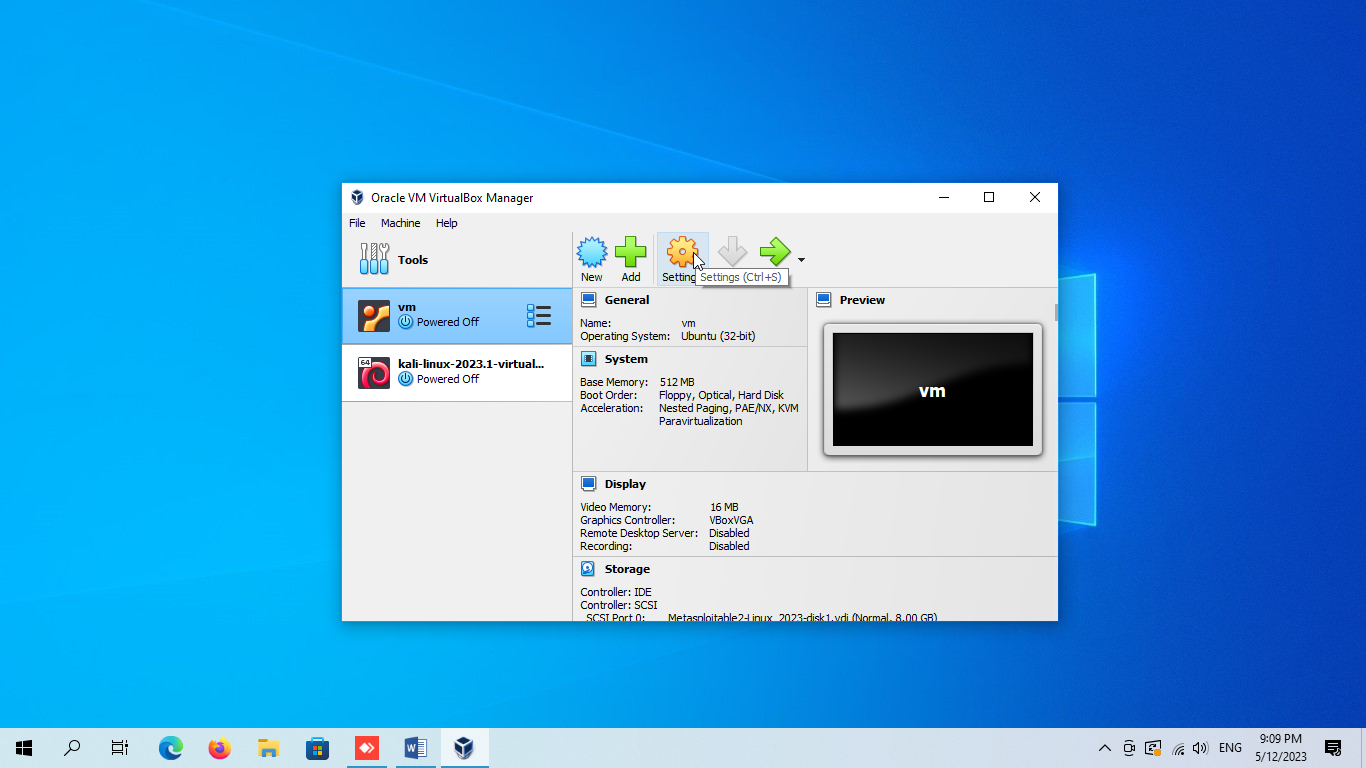
\includegraphics[width=0.85\textwidth]{04_0010}
    \label{img:6}
    \caption{Открываем настройки нужной ВМ}
  \end{figure}

  \begin{figure}[H]
    \centering
    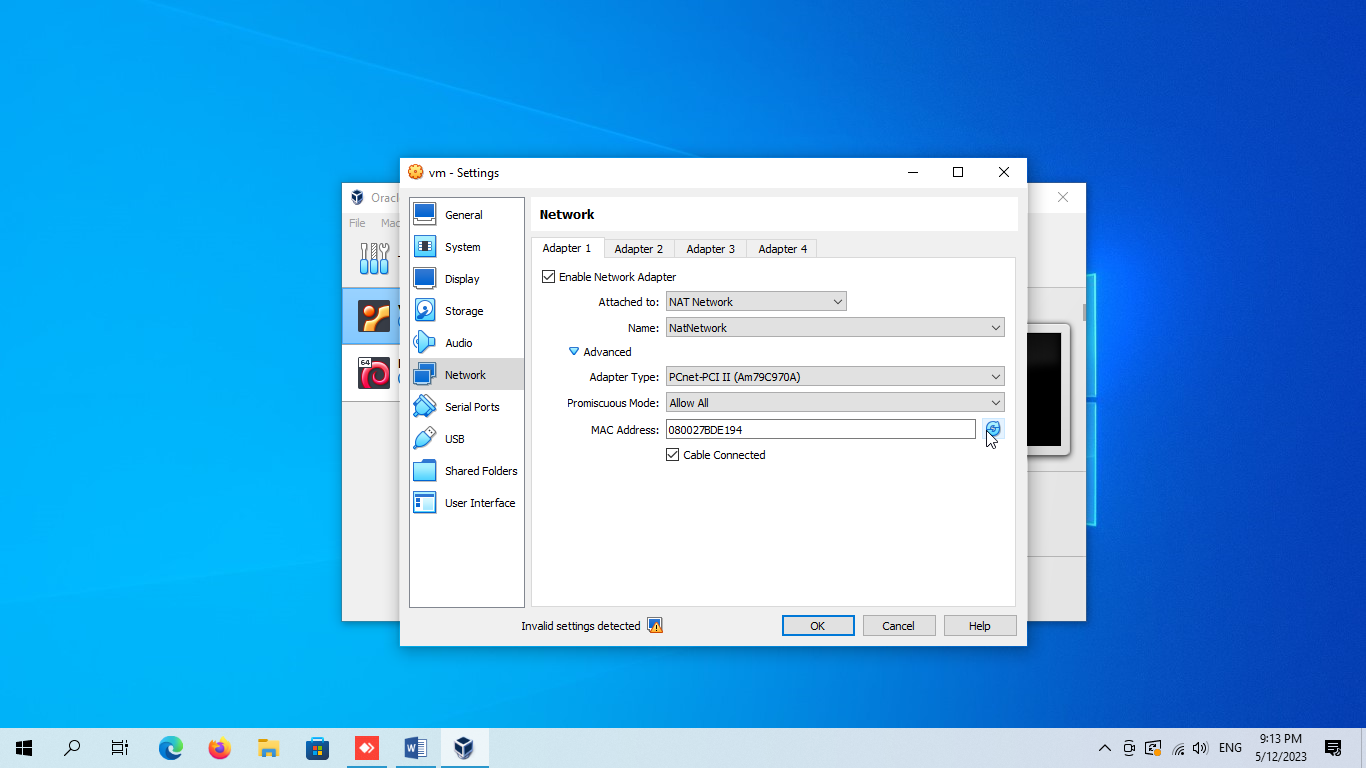
\includegraphics[width=0.85\textwidth]{04_0031}
    \label{img:7}
    \caption{Подключаем сетевой адаптер к нужной сети}
  \end{figure}

  Теперь атакуемая машина настроена и готова к работе, создадим атакующую.
  Будем использовать \textit{Kali Linux}, в базовой установке которого уже имеются
  необходимые для выполнения данной работы инструменты.

  Скачиваем специальный образ с официального сайта и импортируем его:

  \begin{figure}[H]
    \centering
    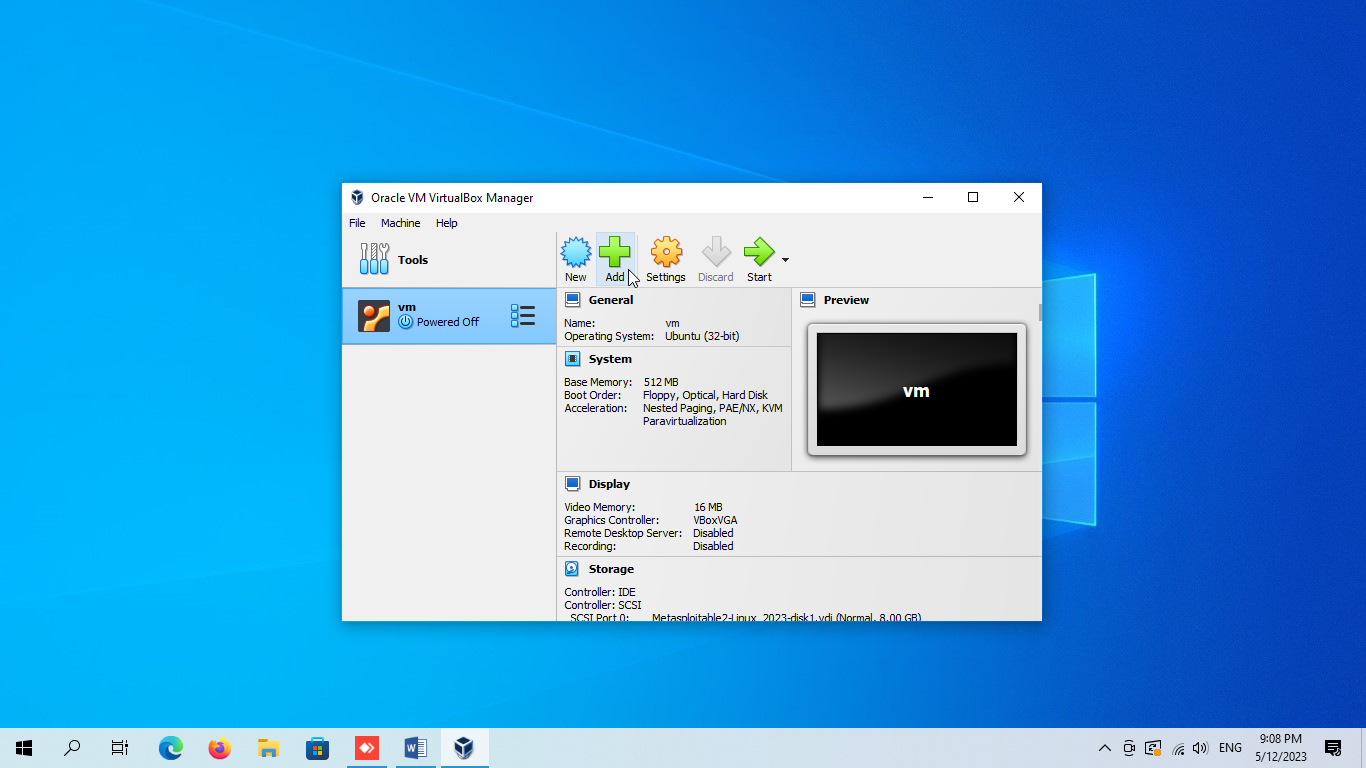
\includegraphics[width=0.85\textwidth]{04_0008}
    \label{img:8}
    \caption{Добавляем новую ВМ}
  \end{figure}

  \begin{figure}[H]
    \centering
    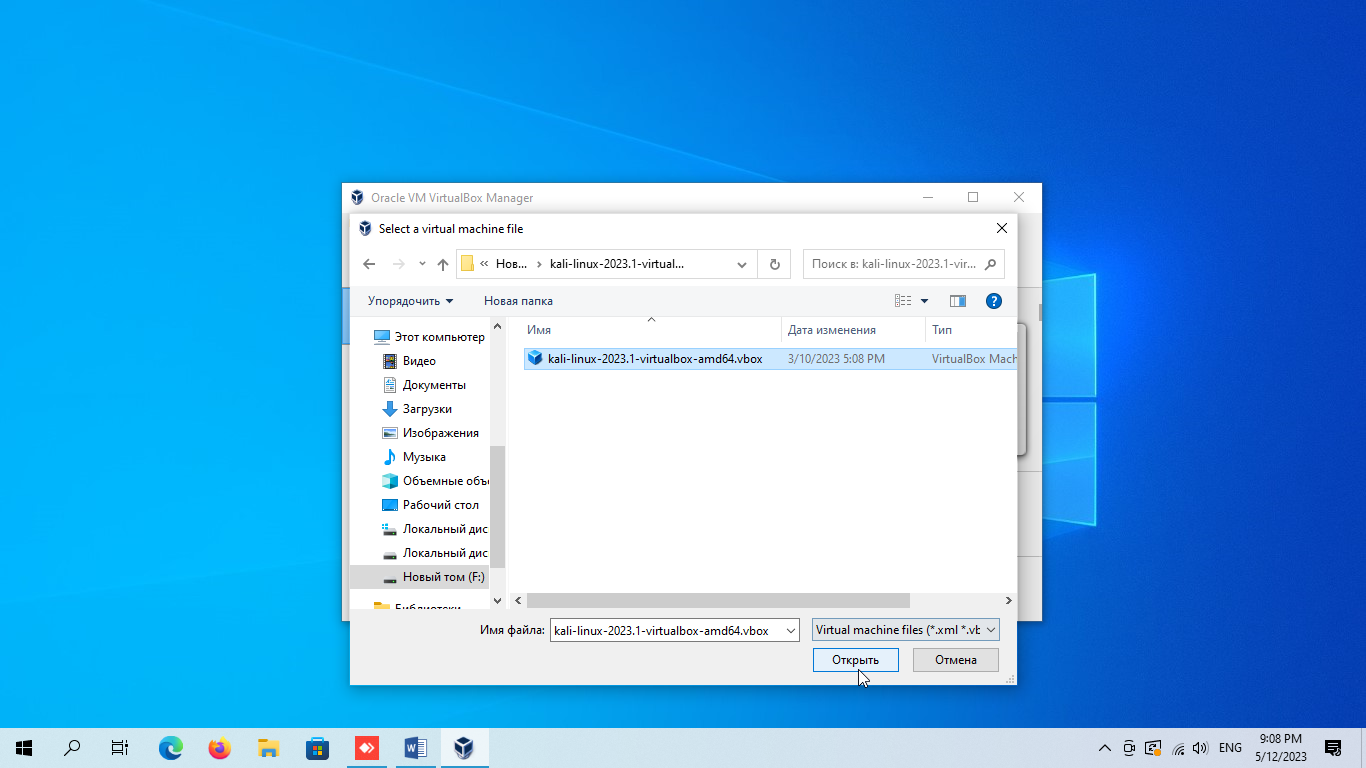
\includegraphics[width=0.85\textwidth]{04_0009}
    \label{img:9}
    \caption{Указываем путь до образа с системой}
  \end{figure}

  Атакующую машину также необходимо подключить к правильной сети:

  \begin{figure}[H]
    \centering
    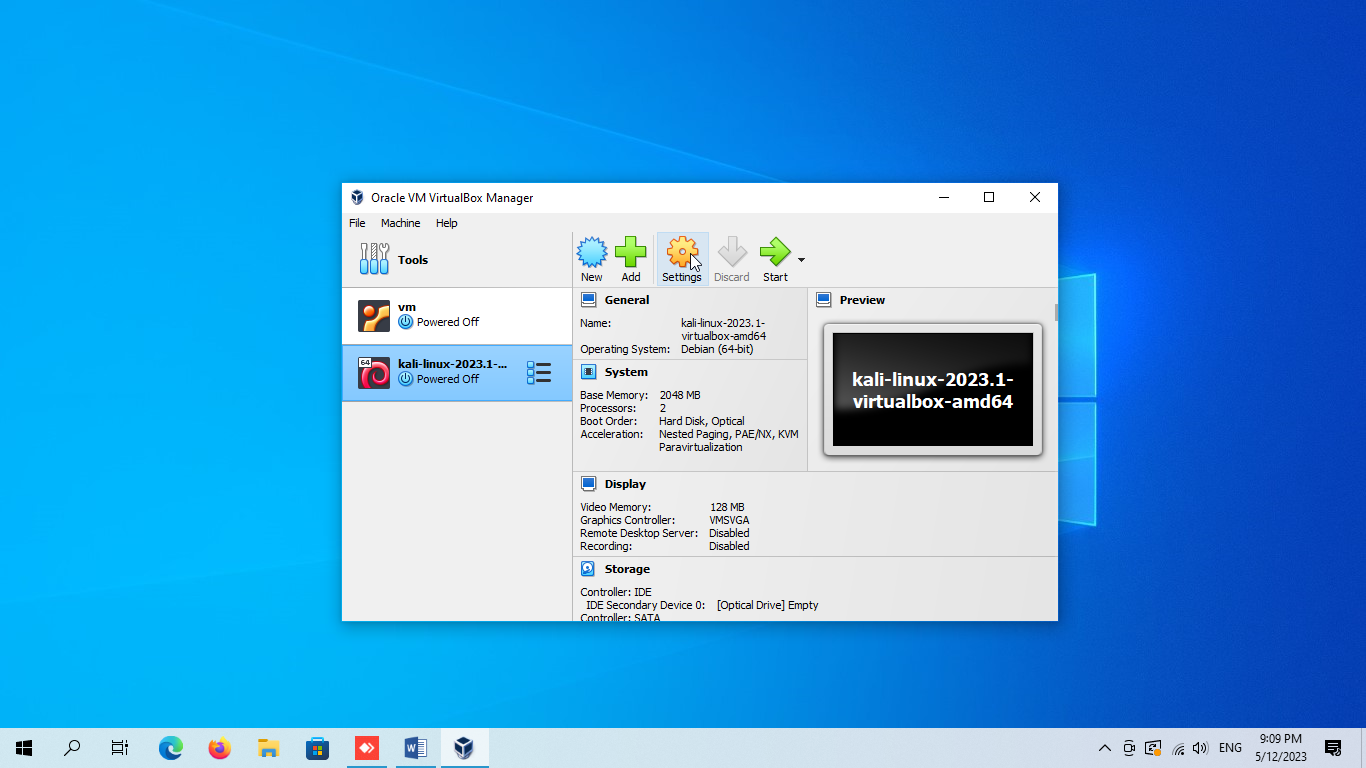
\includegraphics[width=0.85\textwidth]{04_0015}
    \label{img:10}
    \caption{Открываем настройки ВМ}
  \end{figure}

  \begin{figure}[H]
    \centering
    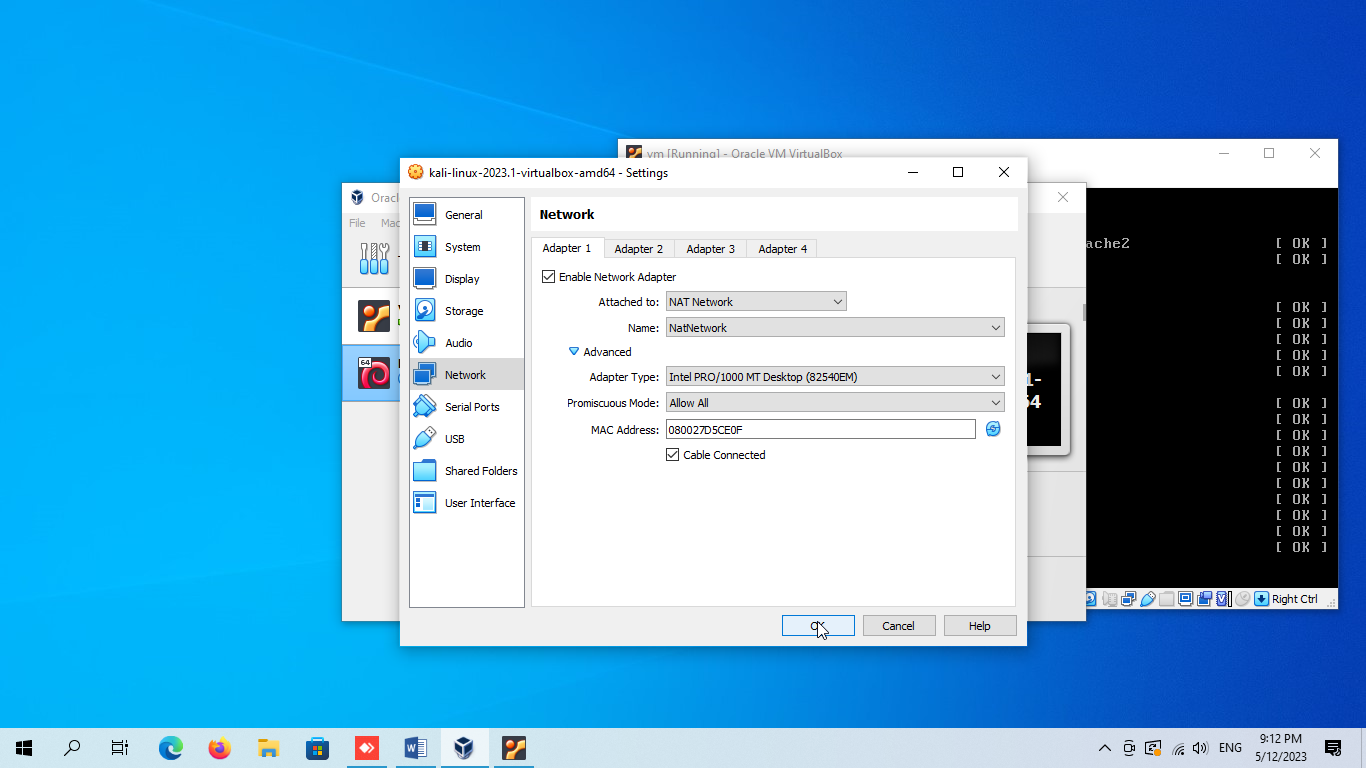
\includegraphics[width=0.85\textwidth]{04_0030}
    \label{img:11}
    \caption{Указываем необходимую сеть}
  \end{figure}

  Теперь настроена и атакующая машина. Запустим обе и узнаем информацию об их сетевых интерфейсах:

  \begin{figure}[H]
    \centering
    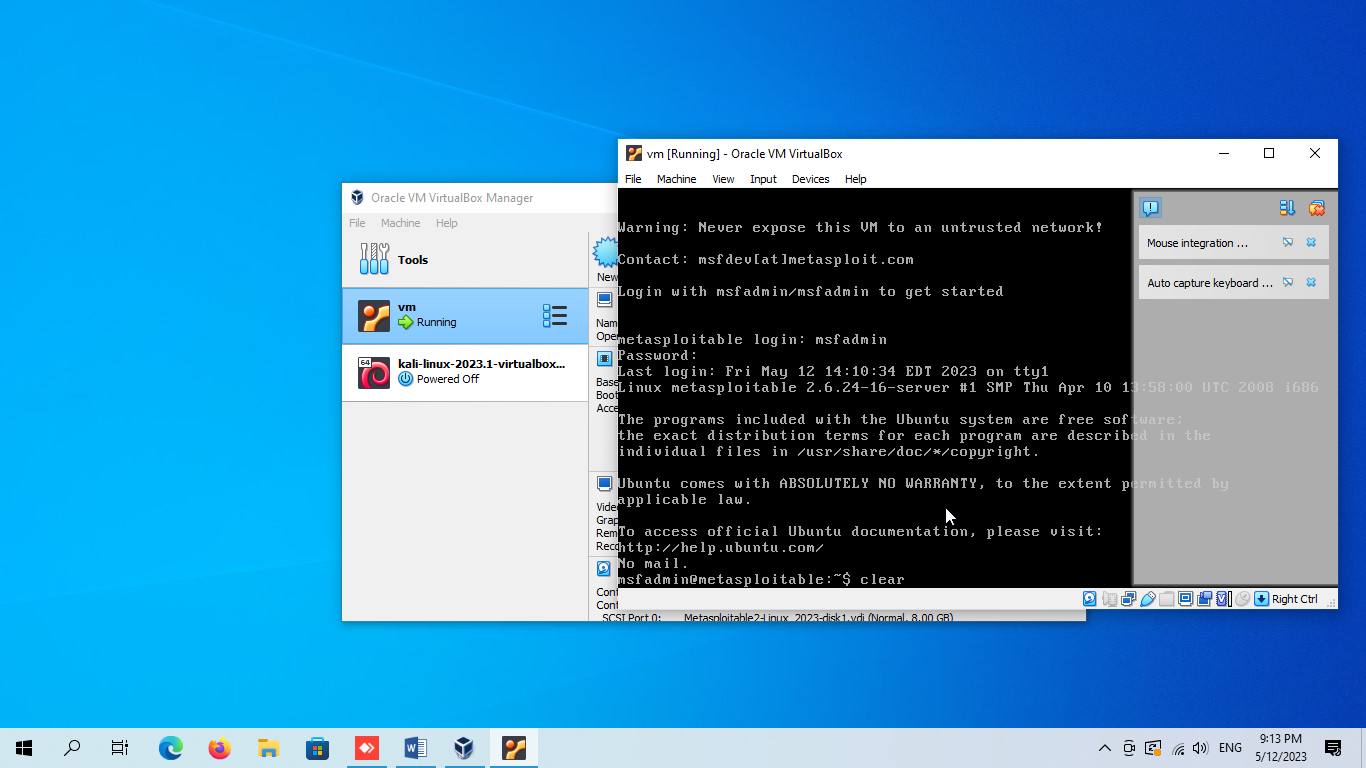
\includegraphics[width=0.85\textwidth]{04_0032}
    \label{img:12}
    \caption{Запуск атакуемой машины, вход в учетную запись пользователя}
  \end{figure}

  \begin{figure}[H]
    \centering
    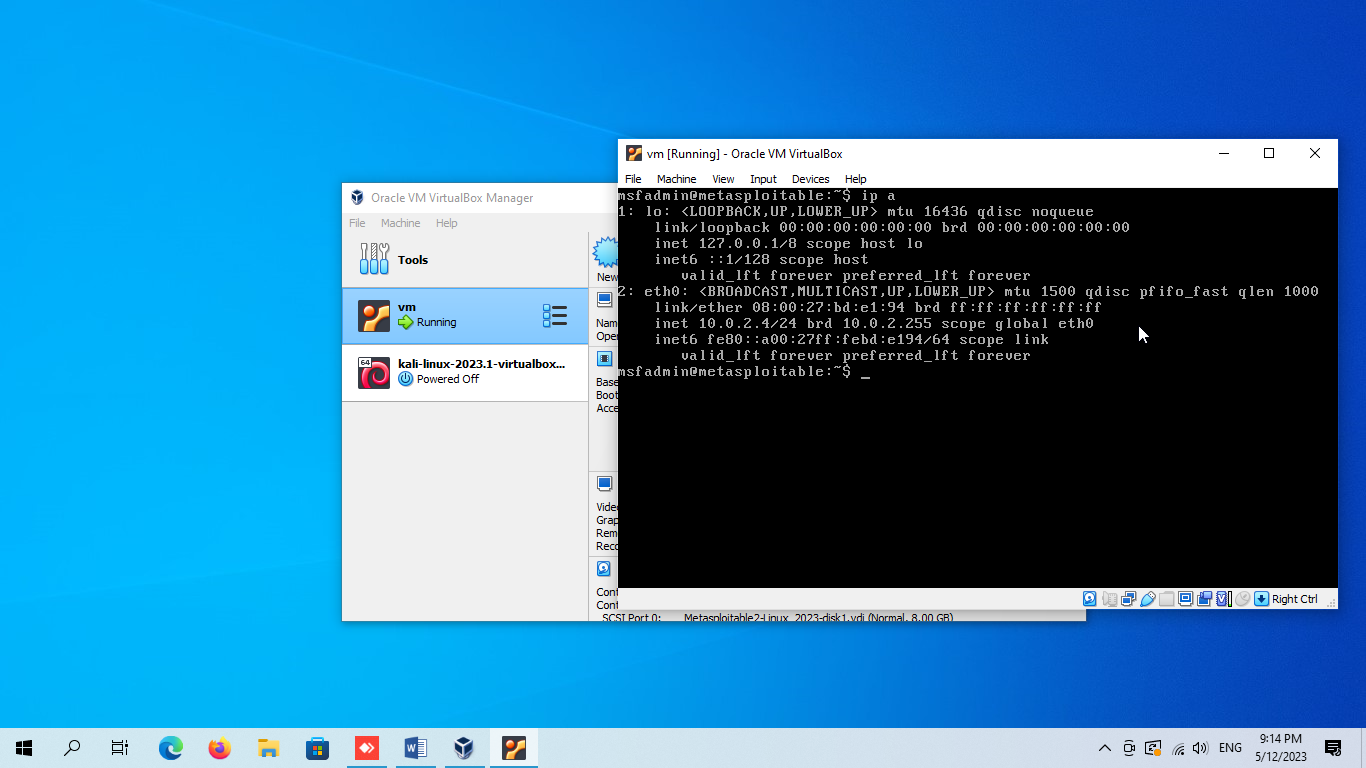
\includegraphics[width=0.85\textwidth]{04_0033}
    \label{img:13}
    \caption{Информация о сетевых настройках атакуемой машины - утилита \textit{ip}}
  \end{figure}
  \begin{figure}[H]
    \centering
    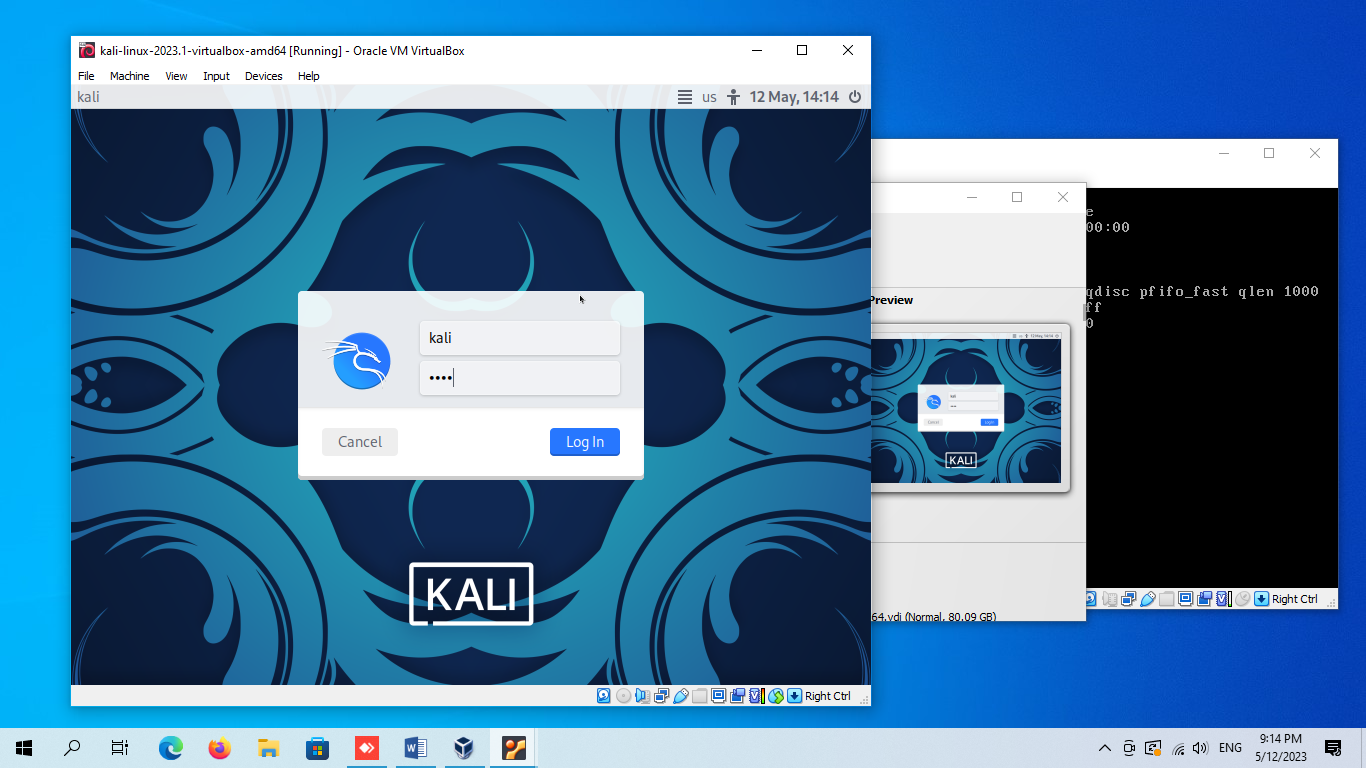
\includegraphics[width=0.85\textwidth]{04_0034}
    \label{img:34}
    \caption{Запуск атакующей машины - вход в учетную запись}
  \end{figure}

  \begin{figure}[H]
    \centering
    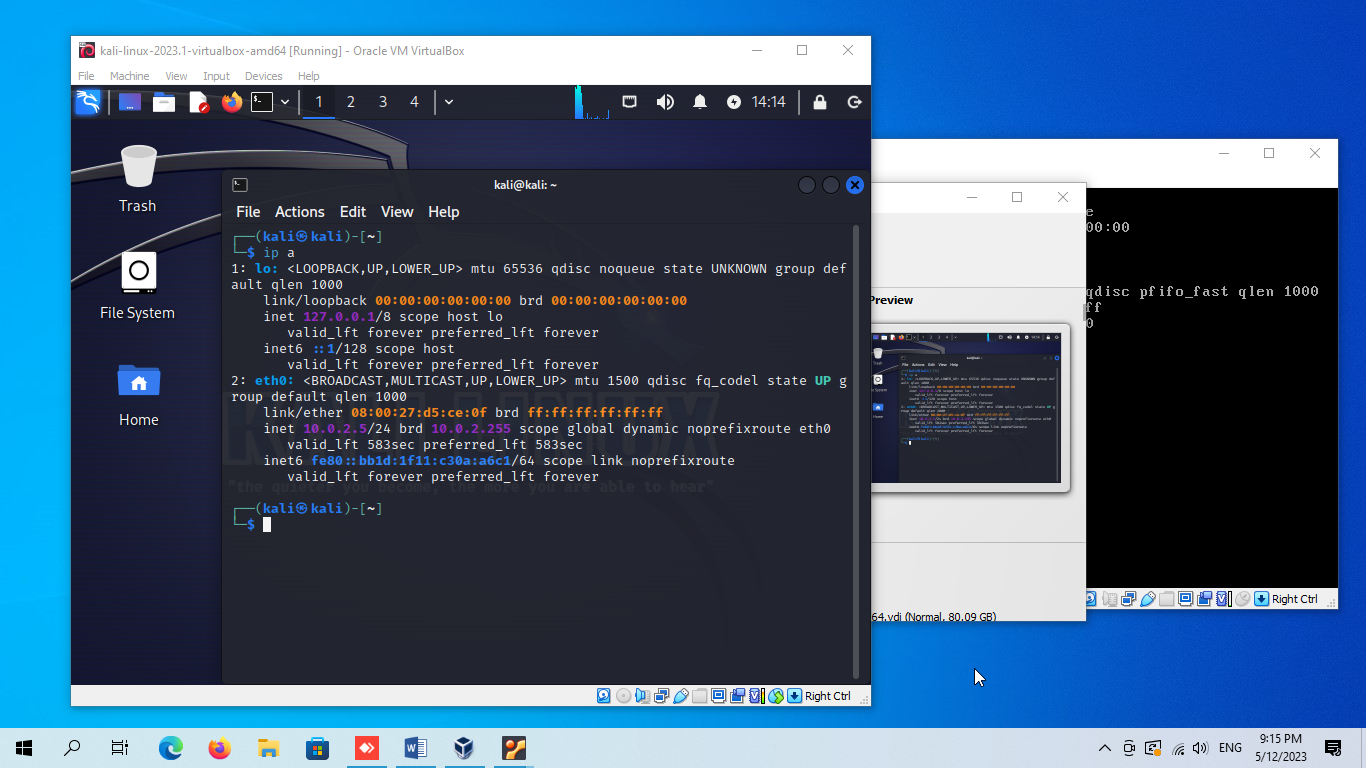
\includegraphics[width=0.85\textwidth]{04_0036}
    \label{img:36}
    \caption{Информация о сетевых интерфейсах атакующей машины}
  \end{figure}

  Вынесем полученную информацию в таблицу:
  \begin{table}[H]
    \centering
    \begin{tabular}{|c|c|c|}
        \hline
        Машина & IPv4 & MAC \\
        \hline
        Атакуемая & 10.0.2.4 & 08:00:27:bd:e1:94 \\
        \hline
        Атакующая & 10.0.2.5 & 08:00:27:d5:ce:0f \\
        \hline
    \end{tabular}
  \end{table}

  Проверим, что каждая машина может достучаться по сети до другой при помощи встроенной
  утилиты \textit{ping}:

  \begin{figure}[H]
    \centering
    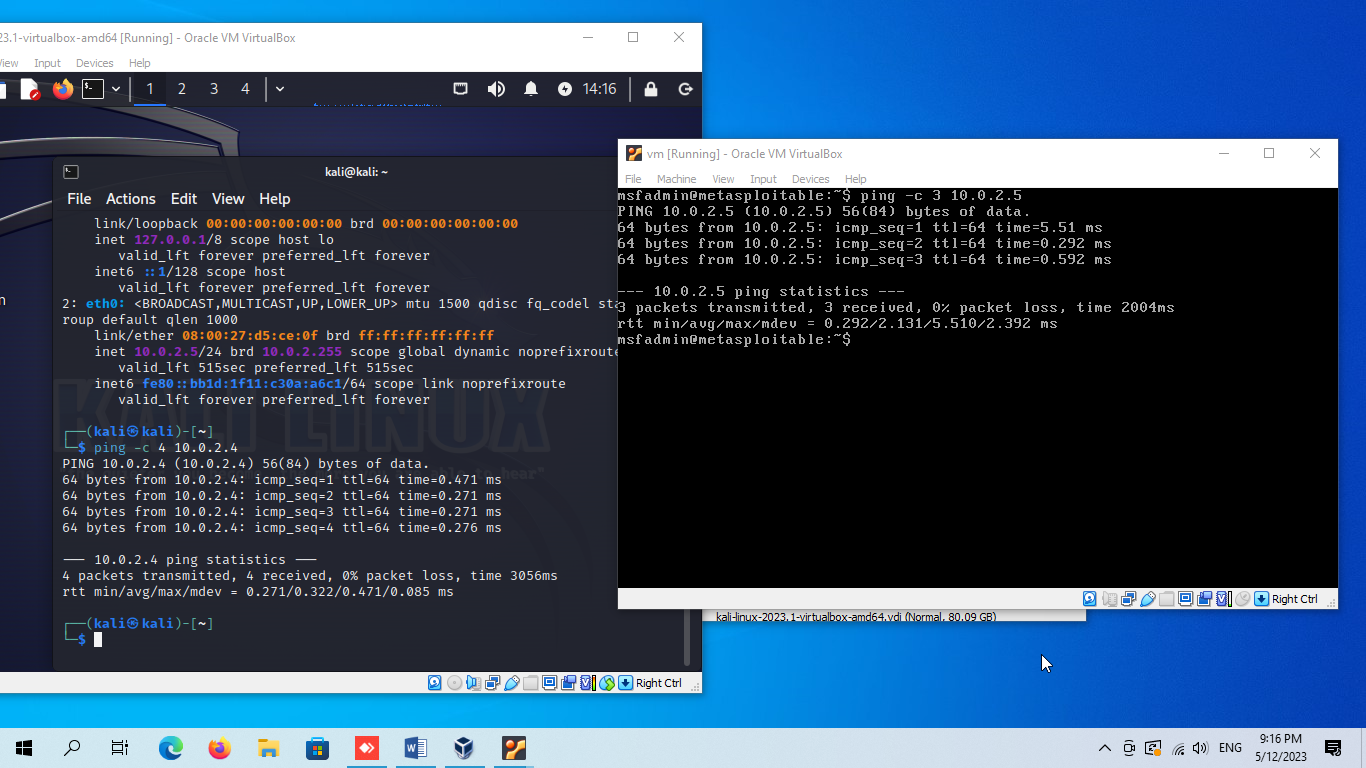
\includegraphics[width=0.85\textwidth]{04_0037}
    \label{img:37}
    \caption{Перекрестный \textit{ping}}
  \end{figure}

  \subsection{Сбор информации об атакуемой машине}

  Теперь, зная \textit{IP} адрес атакуемой машины, необходимо ее просканировать,
  чтобы понять, какие потенциальный уязвимости можно заэксплуатировать.

  Для этого проинициализируем базу данных \textit{Metaspoit Framework} и запустим его: 

  \begin{figure}[H]
    \centering
    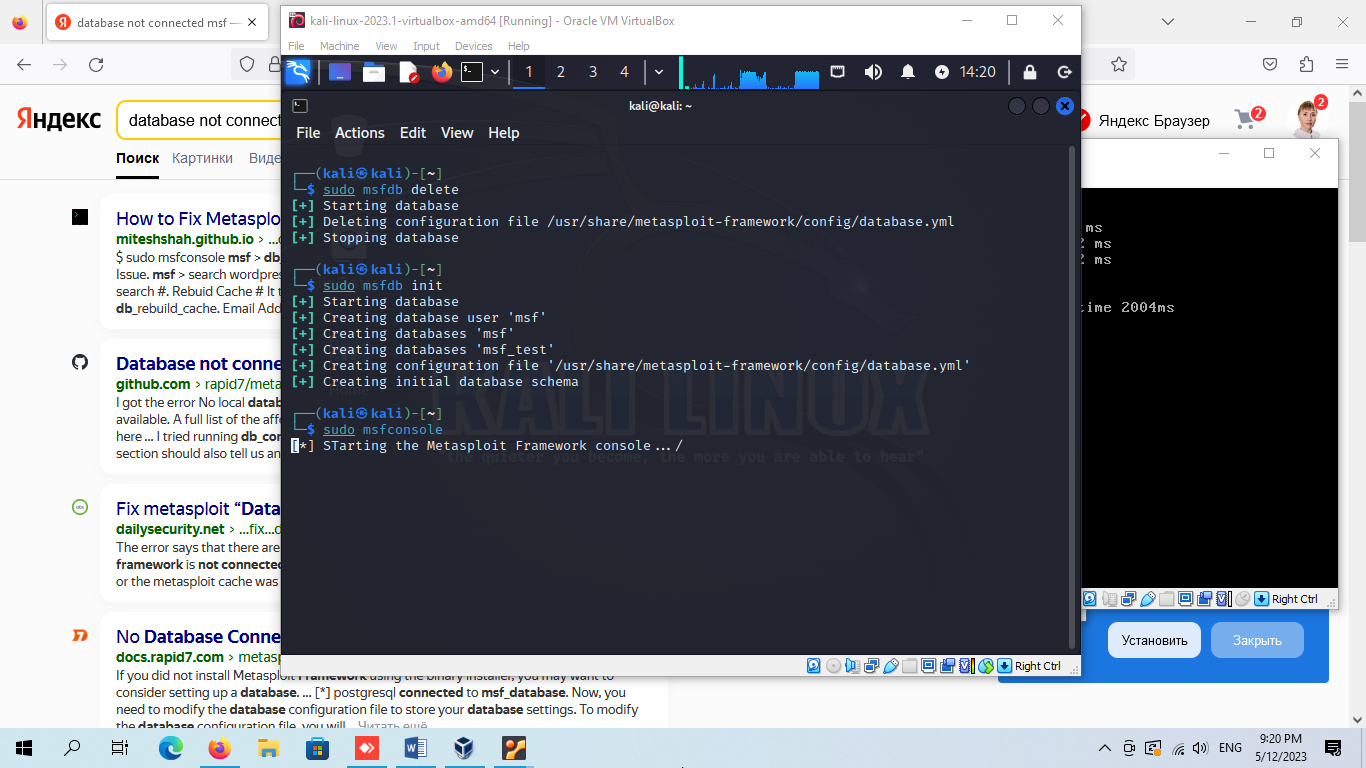
\includegraphics[width=0.85\textwidth]{04_0043}
    \label{img:43}
    \caption{Инициализация базы уязвимостей и запуск \textit{MSF}}
  \end{figure}

  \begin{figure}[H]
    \centering
    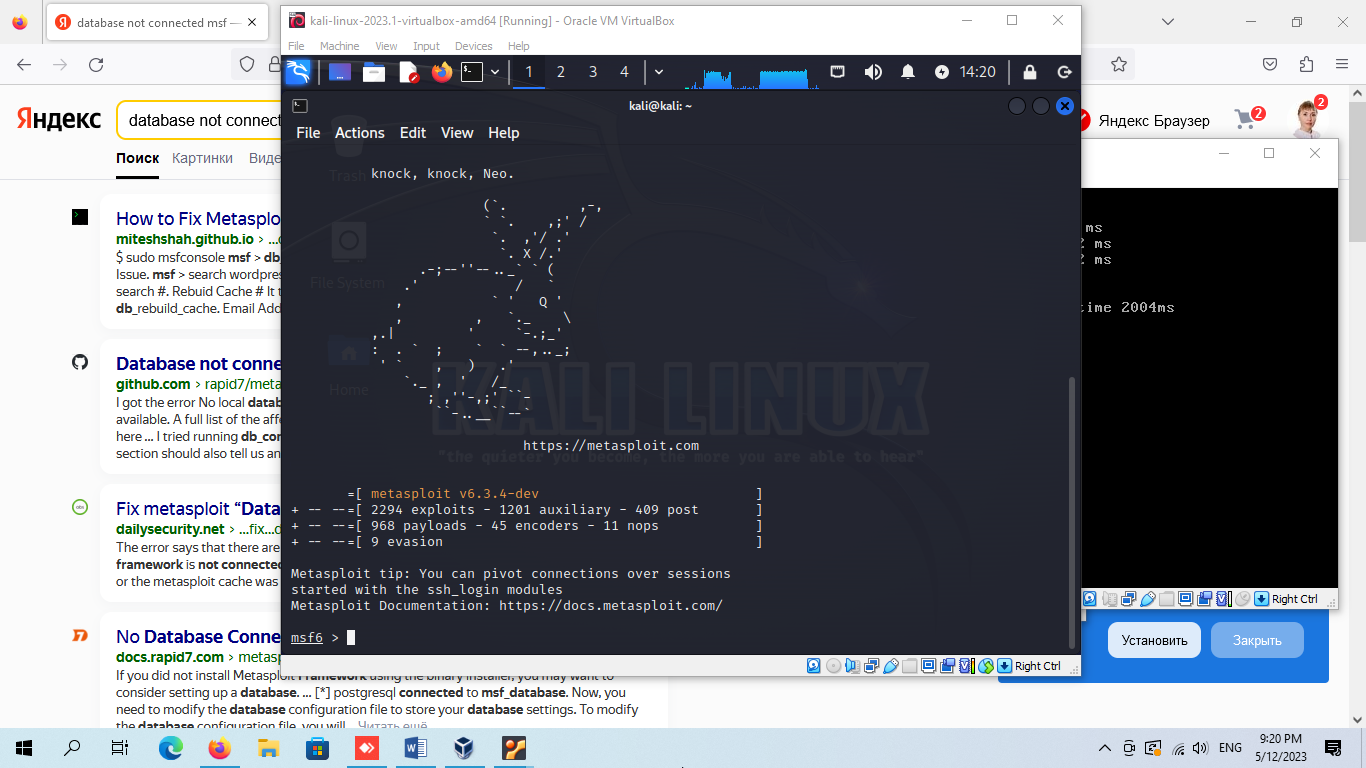
\includegraphics[width=0.85\textwidth]{04_0044}
    \label{img:44}
    \caption{Запущенный \textit{Metasploit}}
  \end{figure}

  Для сканирования атакуемой машины воспользуемся встроенным в \textit{Metasploit nmap}:
  \begin{minted}{bash}
    db_nmap 10.0.2.4 -p- -sV
  \end{minted}

  \begin{figure}[H]
    \centering
    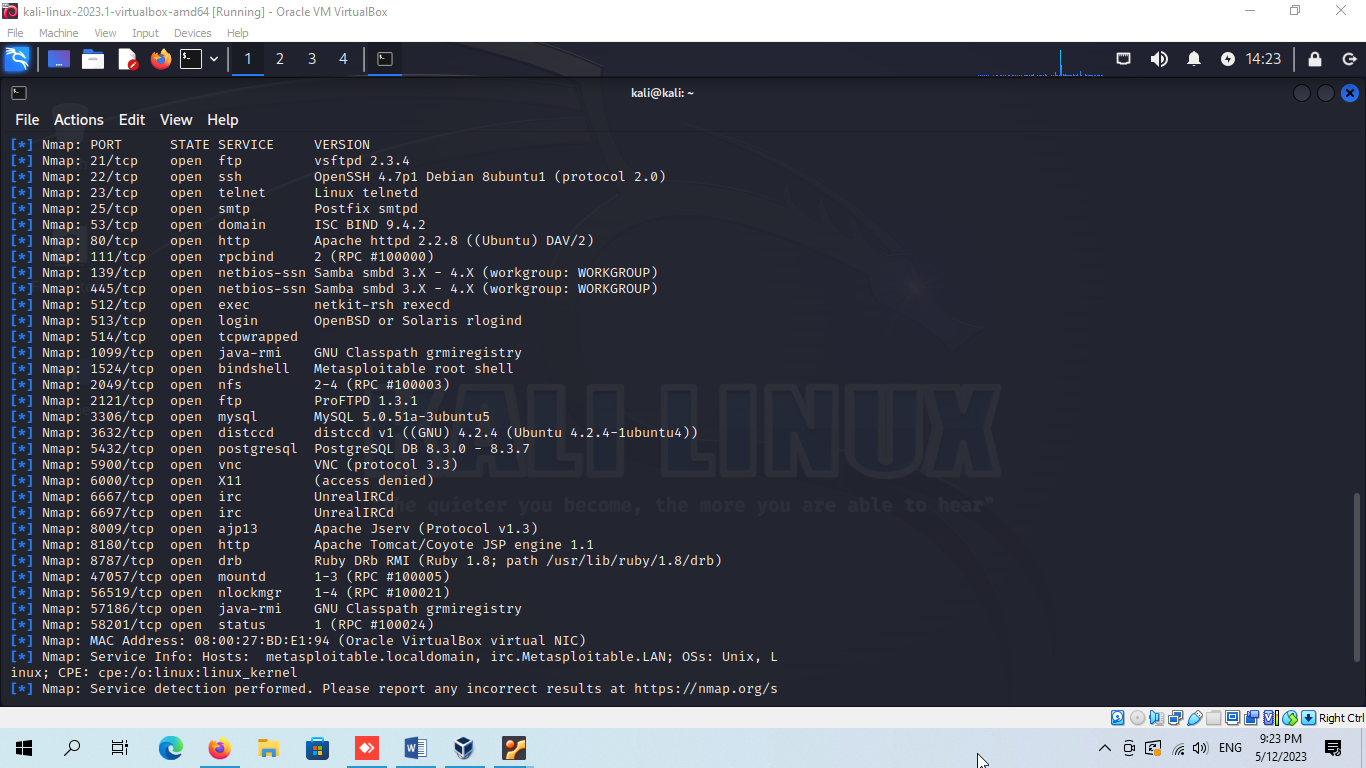
\includegraphics[width=0.85\textwidth]{04_0045}
    \label{img:45}
    \caption{Результаты сканирования}
  \end{figure}

  Результаты сканирования дают понять, что на атакуемой машине запущено множество
  различных сервисов, в каждом из которых может находиться потенциальная уязвимость.

  Сохраним результат сканирования в файл \textit{/home/kali/res2.xml}

  \begin{figure}[H]
    \centering
    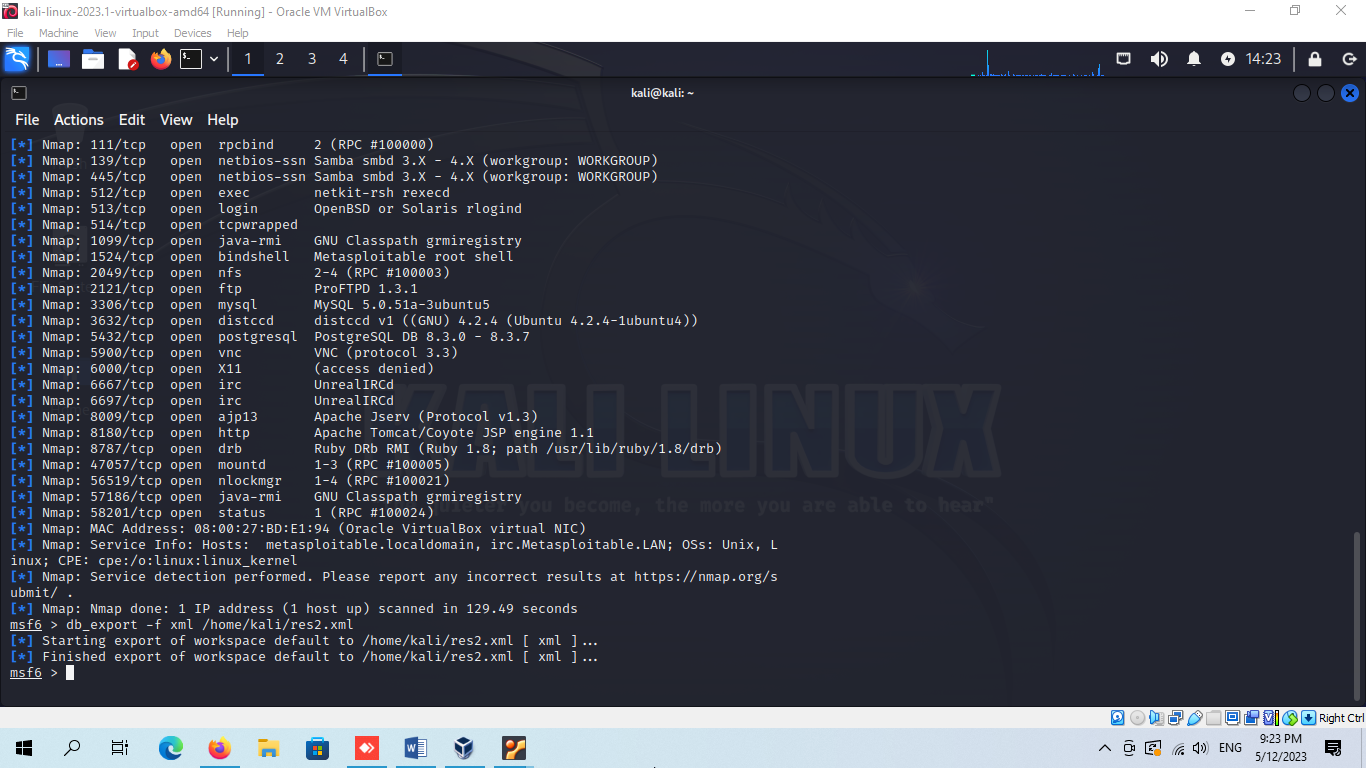
\includegraphics[width=0.85\textwidth]{04_0046}
    \label{img:46}
    \caption{\textit{db\_export} - сохранение результатов сканирования}
  \end{figure}

  Сохраненный \textit{XML} файл можно открыть любой удобной программой и изучить подробнее:

  \begin{figure}[H]
    \centering
    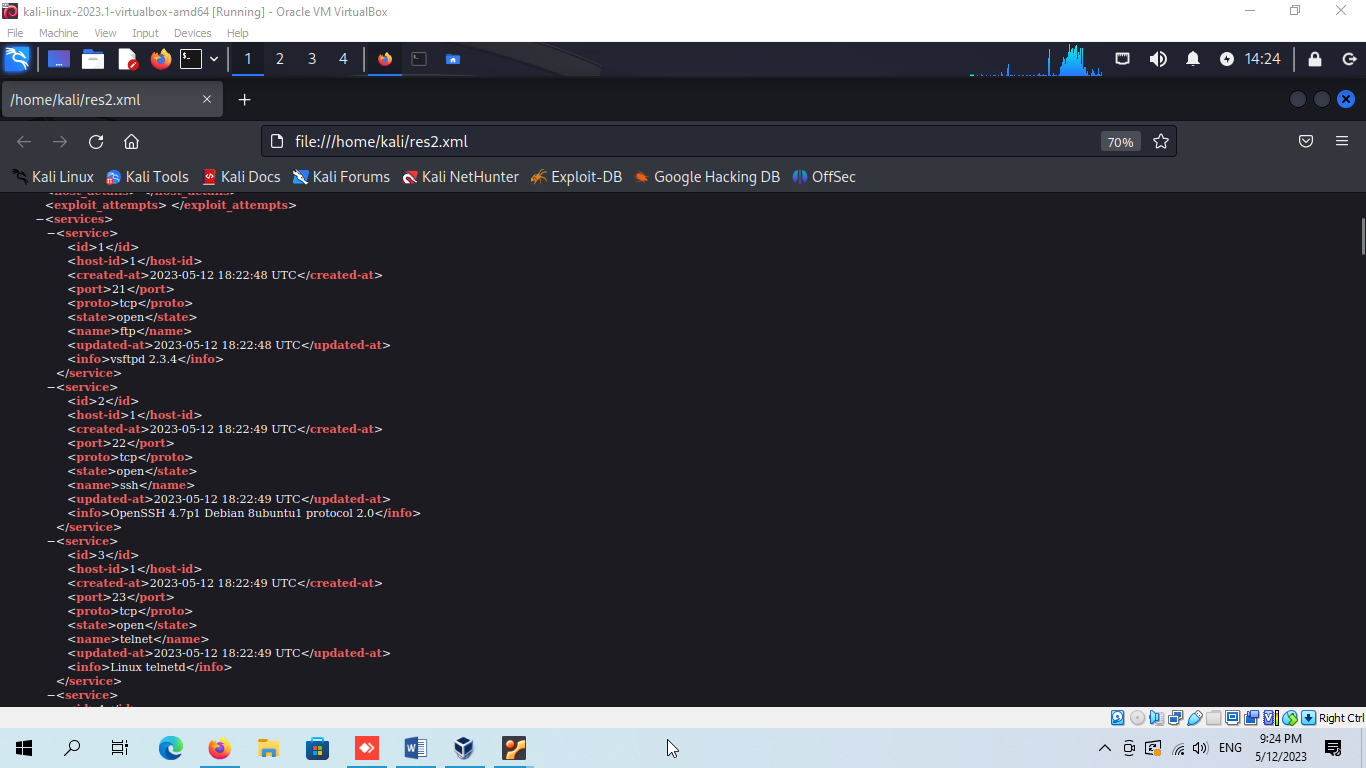
\includegraphics[width=0.85\textwidth]{04_0048}
    \label{img:48}
    \caption{Полученная информация}
  \end{figure}

  \subsection{Подбор паролей}

  Попробуем подобрать пароль к запущенному на атакуемой машине демону
  \textit{PostgreSQL} базы данных, для этого воспользуемся готовым эксплойтом:

  \begin{figure}[H]
    \centering
    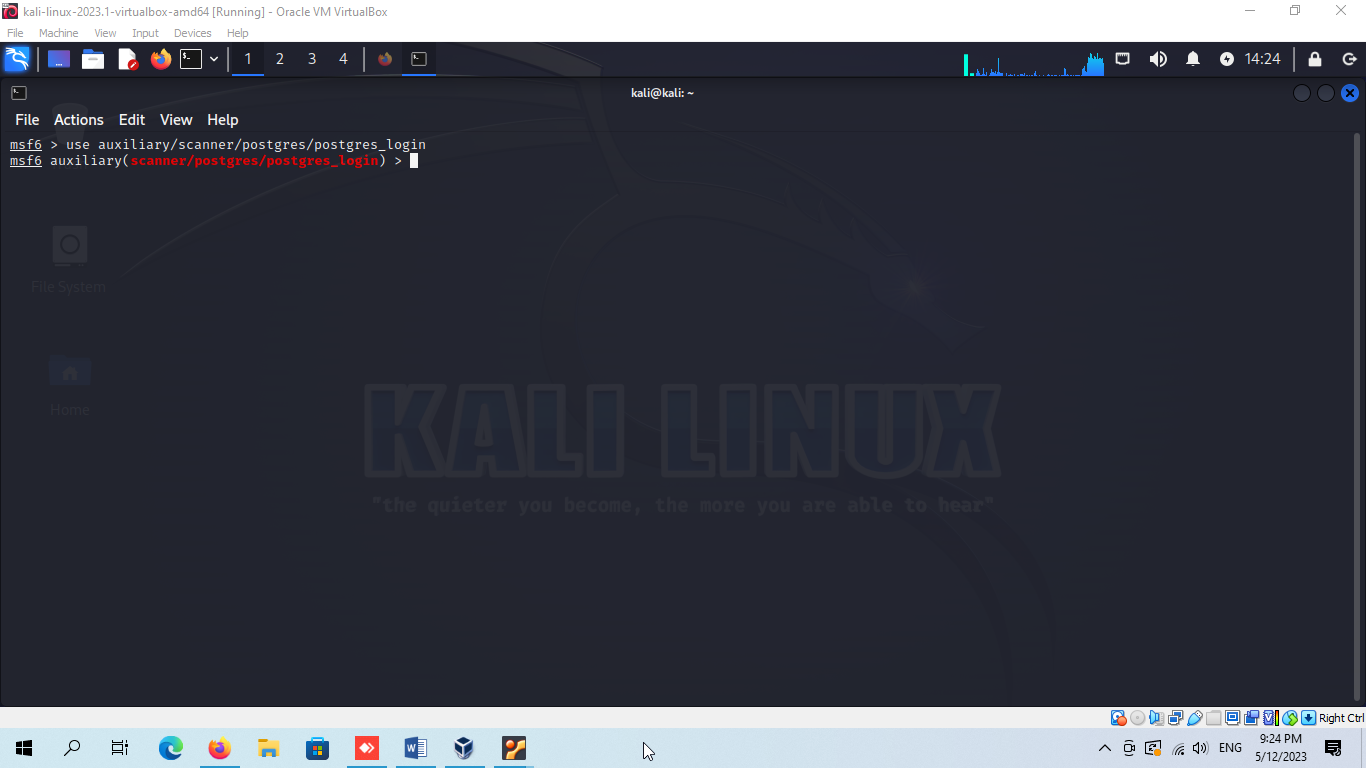
\includegraphics[width=0.85\textwidth]{04_0049}
    \label{img:49}
    \caption{Указываем необходимый эксплойт}
  \end{figure}

  \begin{figure}[H]
    \centering
    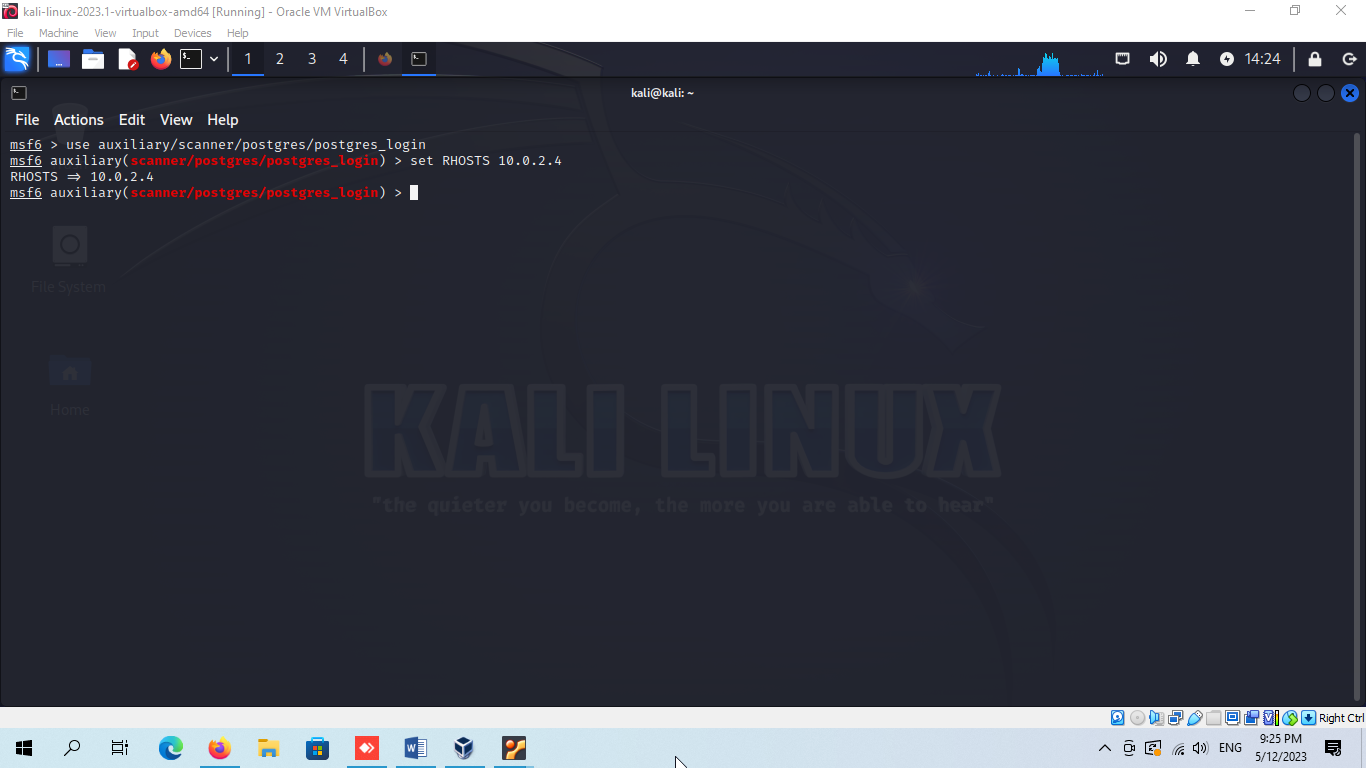
\includegraphics[width=0.85\textwidth]{04_0050}
    \label{img:50}
    \caption{Указываем адрес атакуемой машины}
  \end{figure}

  \begin{figure}[H]
    \centering
    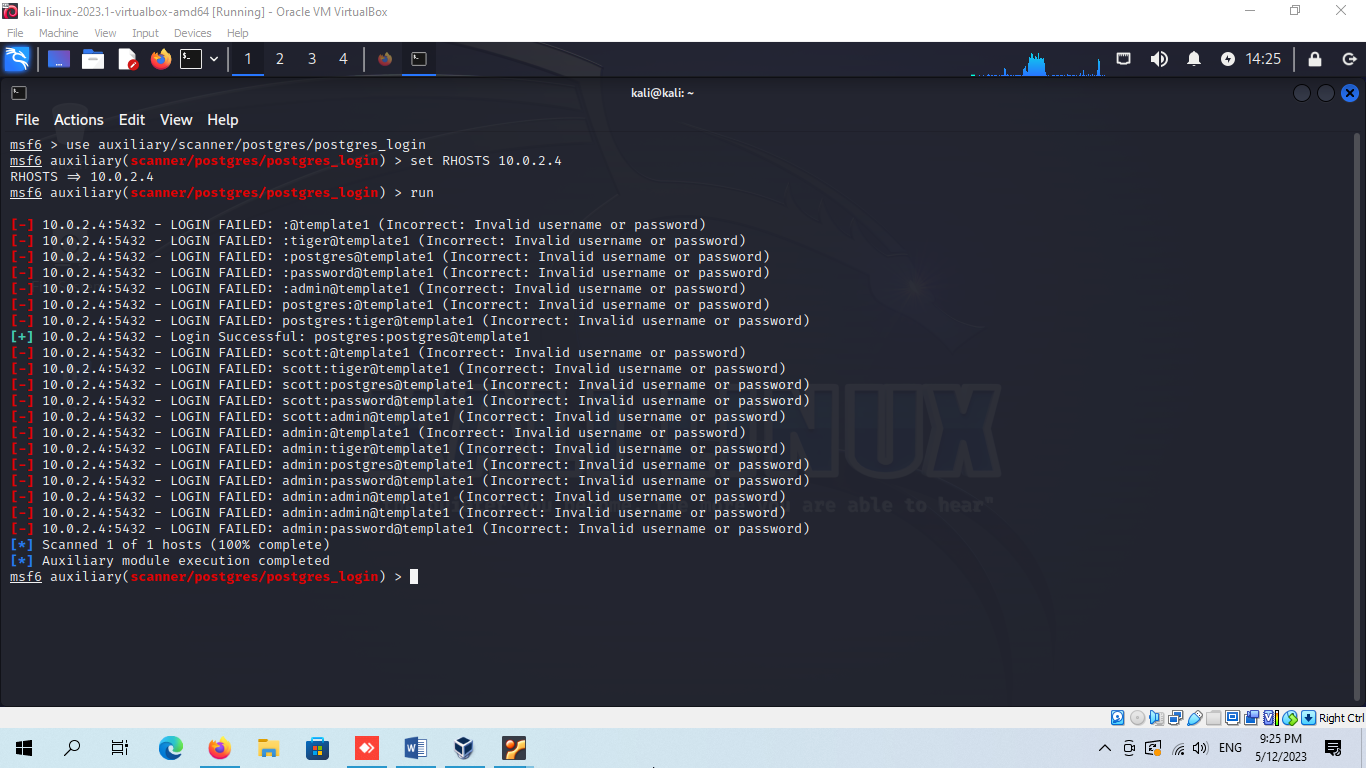
\includegraphics[width=0.85\textwidth]{04_0051}
    \label{img:51}
    \caption{Запускаем атаку}
  \end{figure}

  Видно, что в ходе атаки был найден логин и пароль, с помощью которых можно авторизоваться
  в \textit{psql}. Изучим, какие еще флаги можно задать для конфигурирования данной атаки:

  \begin{figure}[H]
    \centering
    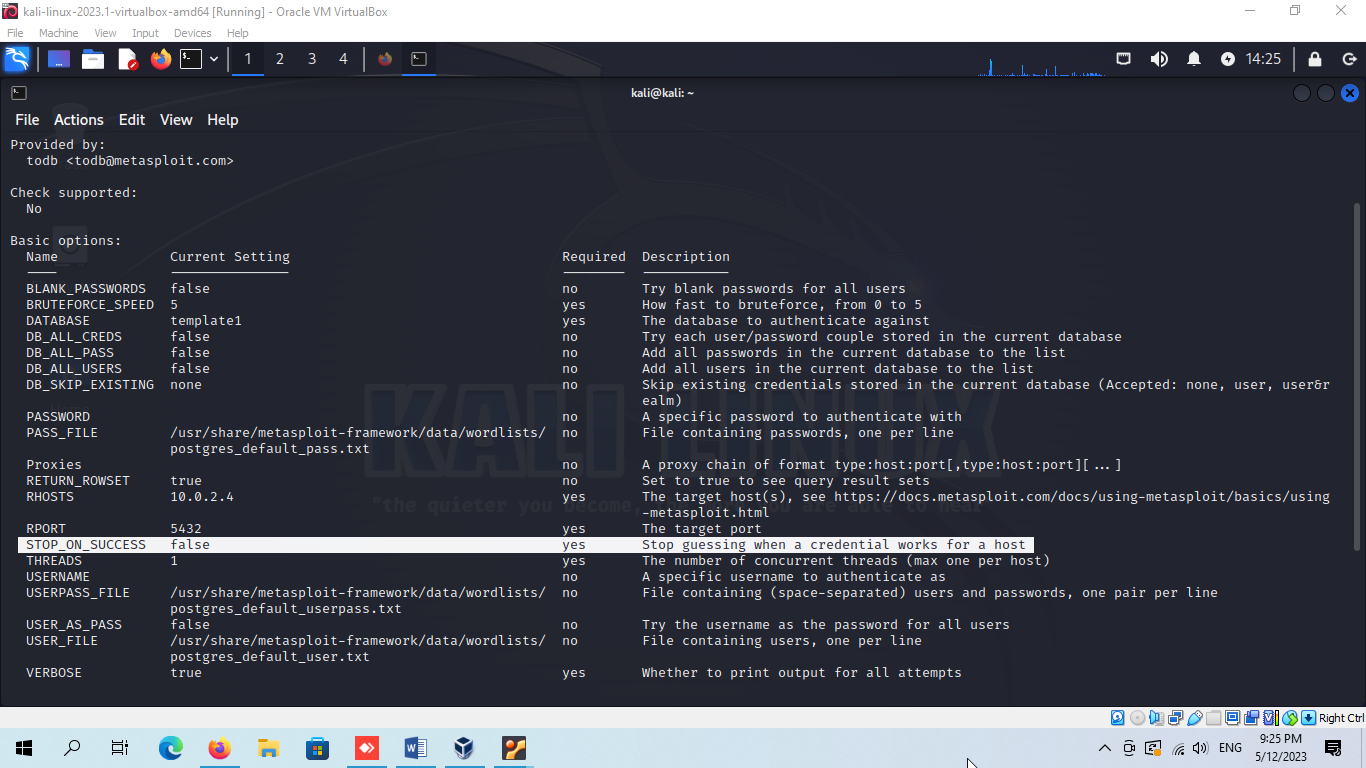
\includegraphics[width=0.85\textwidth]{04_0052}
    \label{img:52}
    \caption{\text{info} - информация об эксплойте}
  \end{figure}

  Интересный параметр \textit{STOP\_ON\_SUCCESS} - останавливает перебор паролей и логинов,
  как только найдет любую подходящую пару. Включим этот флаг и посмотрим на результат:

  \begin{figure}[H]
    \centering
    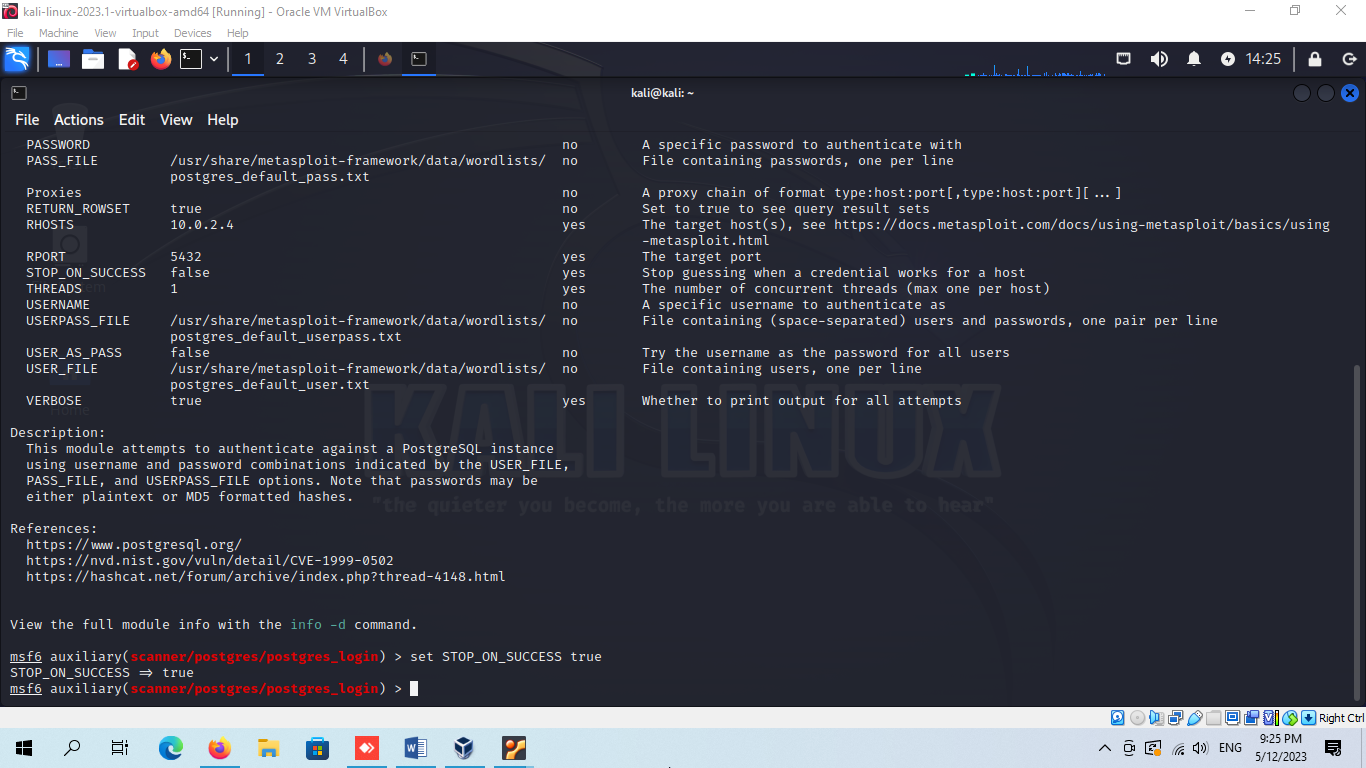
\includegraphics[width=0.85\textwidth]{04_0053}
    \label{img:53}
    \caption{Установка флага}
  \end{figure}

  \begin{figure}[H]
    \centering
    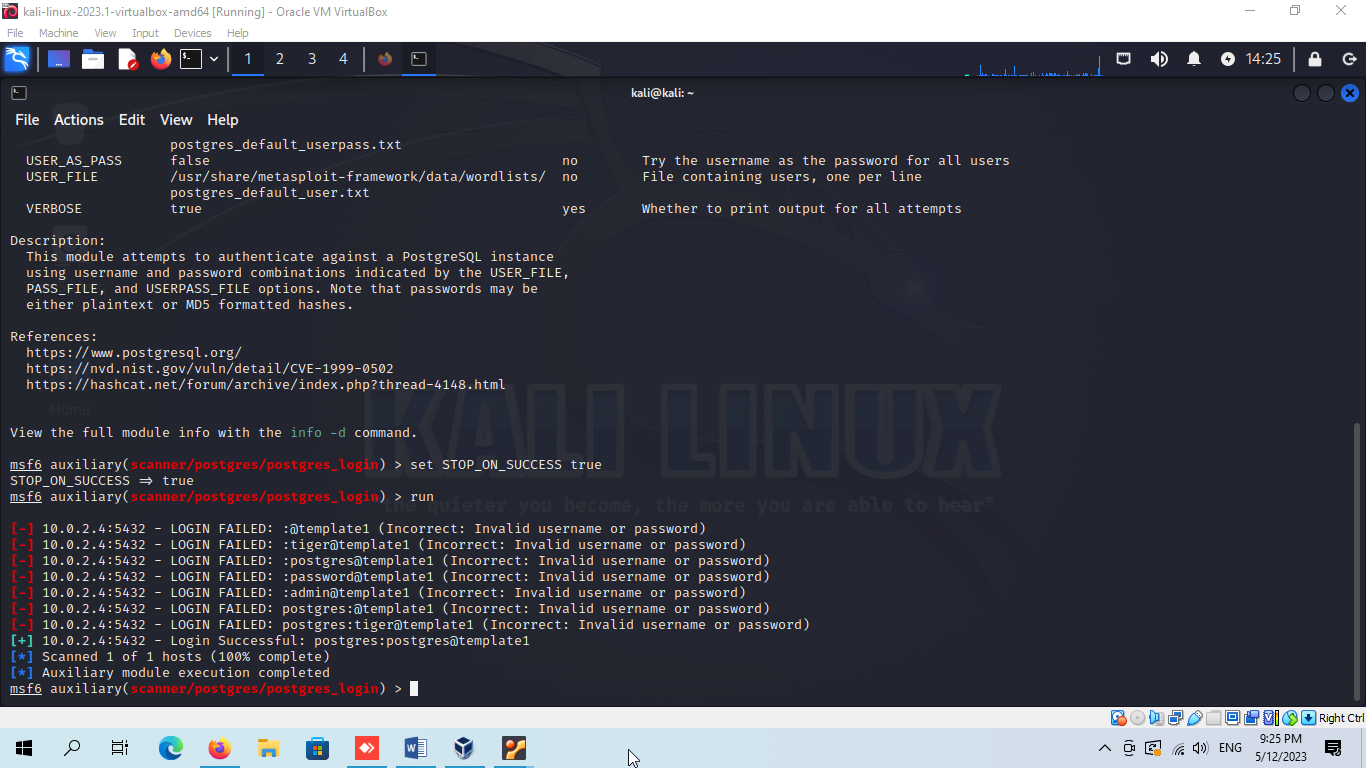
\includegraphics[width=0.85\textwidth]{04_0054}
    \label{img:54}
    \caption{Запуск атаки}
  \end{figure}

  Видно, что атака прекратилась, как только удалось подобрать подходящую пару значений -
  пароль и логин \textit{postgres}.

  Проведем атаку грубой силой на \textit{tomcat}:

  \begin{figure}[H]
    \centering
    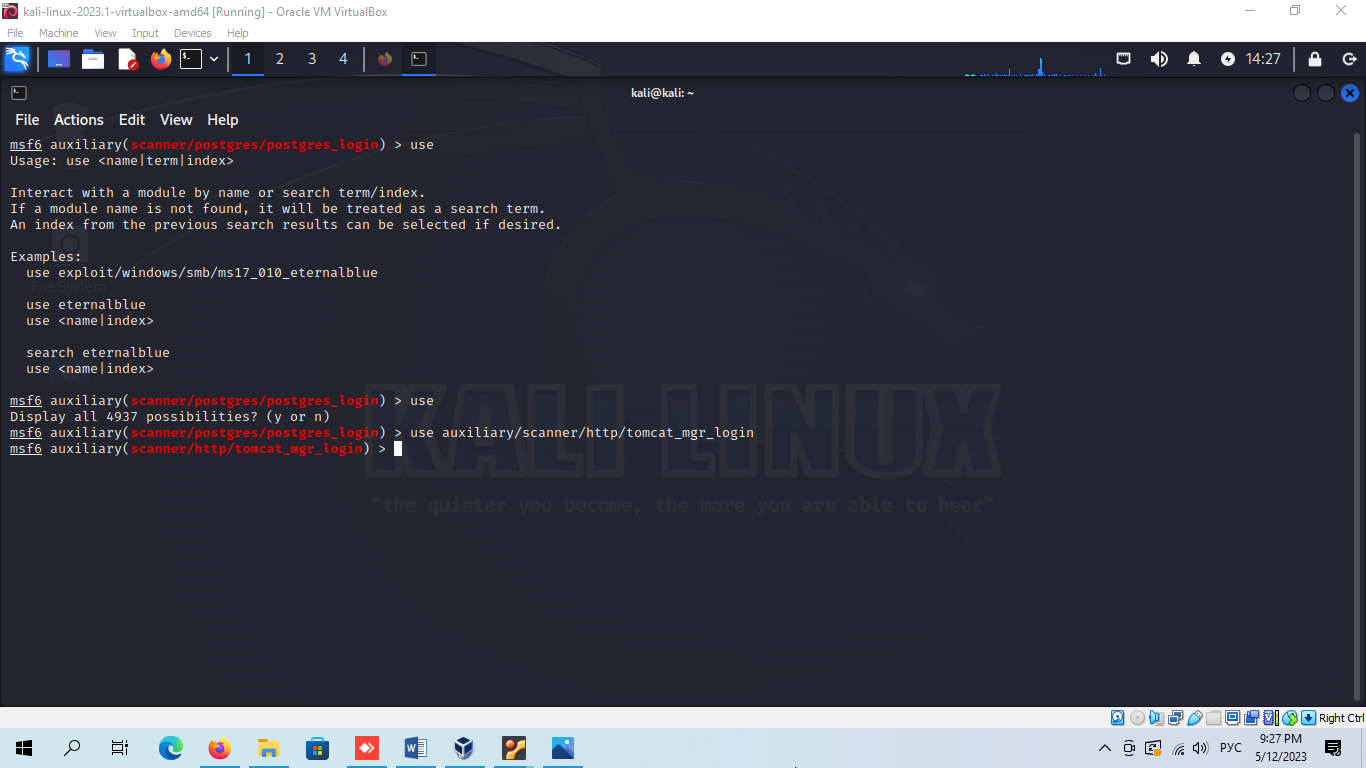
\includegraphics[width=0.85\textwidth]{04_0055}
    \label{img:55}
    \caption{Указываем необходимый эксплойт}
  \end{figure}

  \begin{figure}[H]
    \centering
    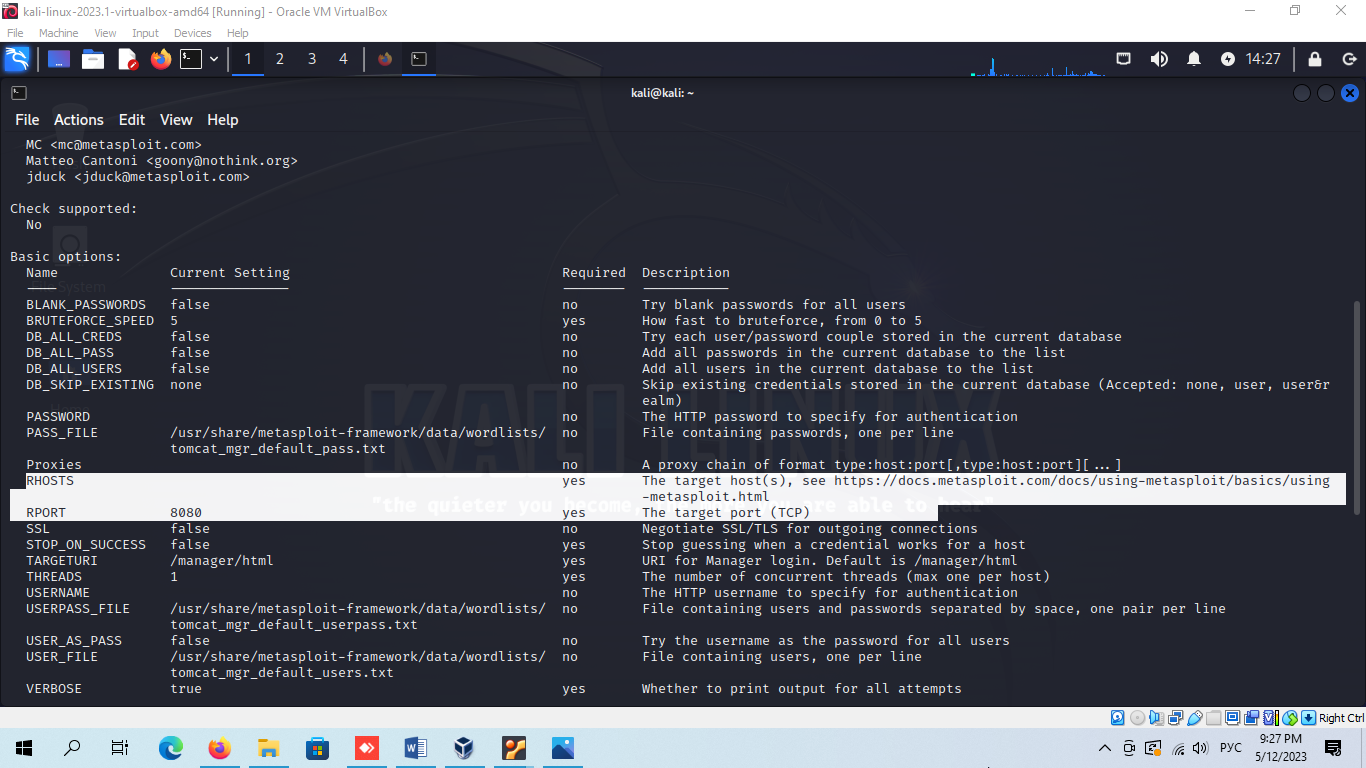
\includegraphics[width=0.85\textwidth]{04_0056}
    \label{img:56}
    \caption{Изучаем параметры данной атаки}
  \end{figure}

  \begin{figure}[H]
    \centering
    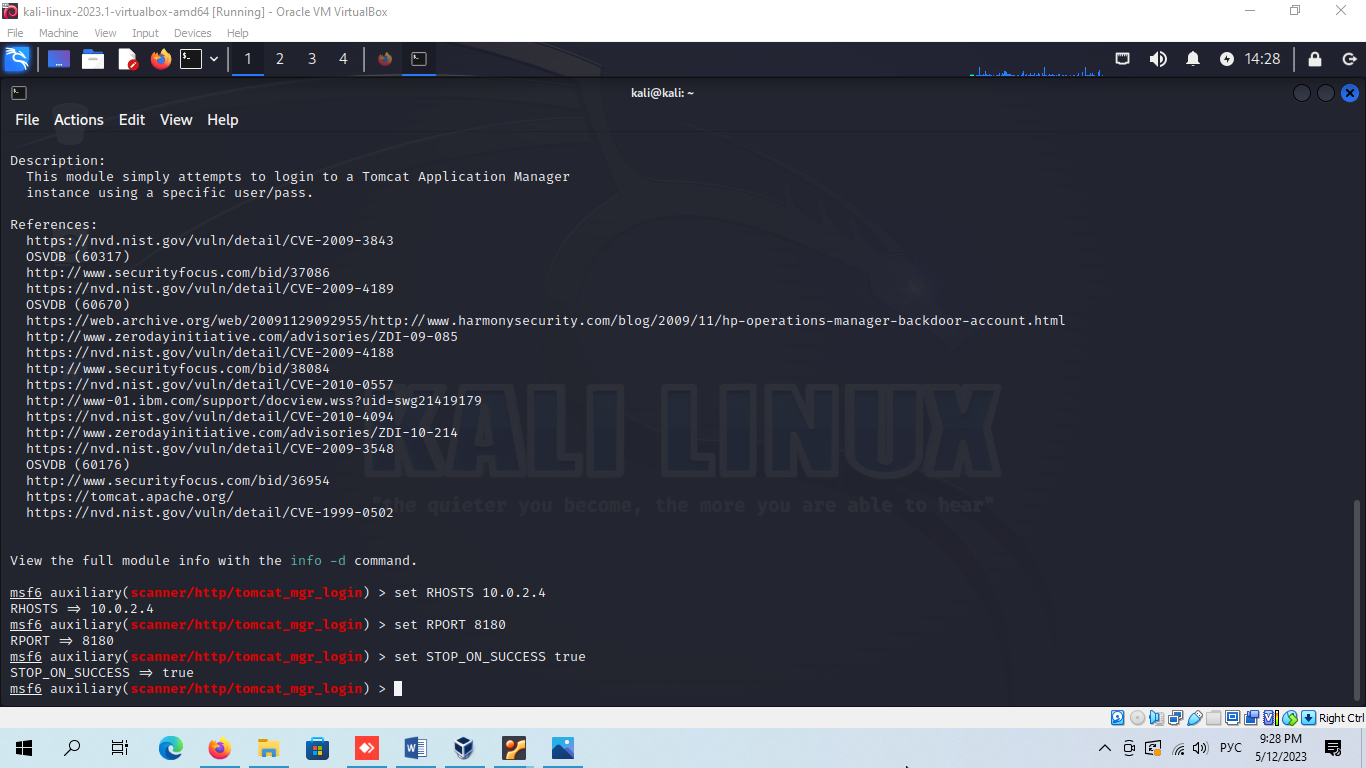
\includegraphics[width=0.85\textwidth]{04_0057}
    \label{img:57}
    \caption{Устанавливаем адрес атакуемой машины и порт для атаки}
  \end{figure}

  Порт отлитчается от стандартного, это можно заметить в результатах сканирования,
  представленных ранее (по умолчанию используется порт 8080, в нашем случае - 8180).

  \begin{figure}[H]
    \centering
    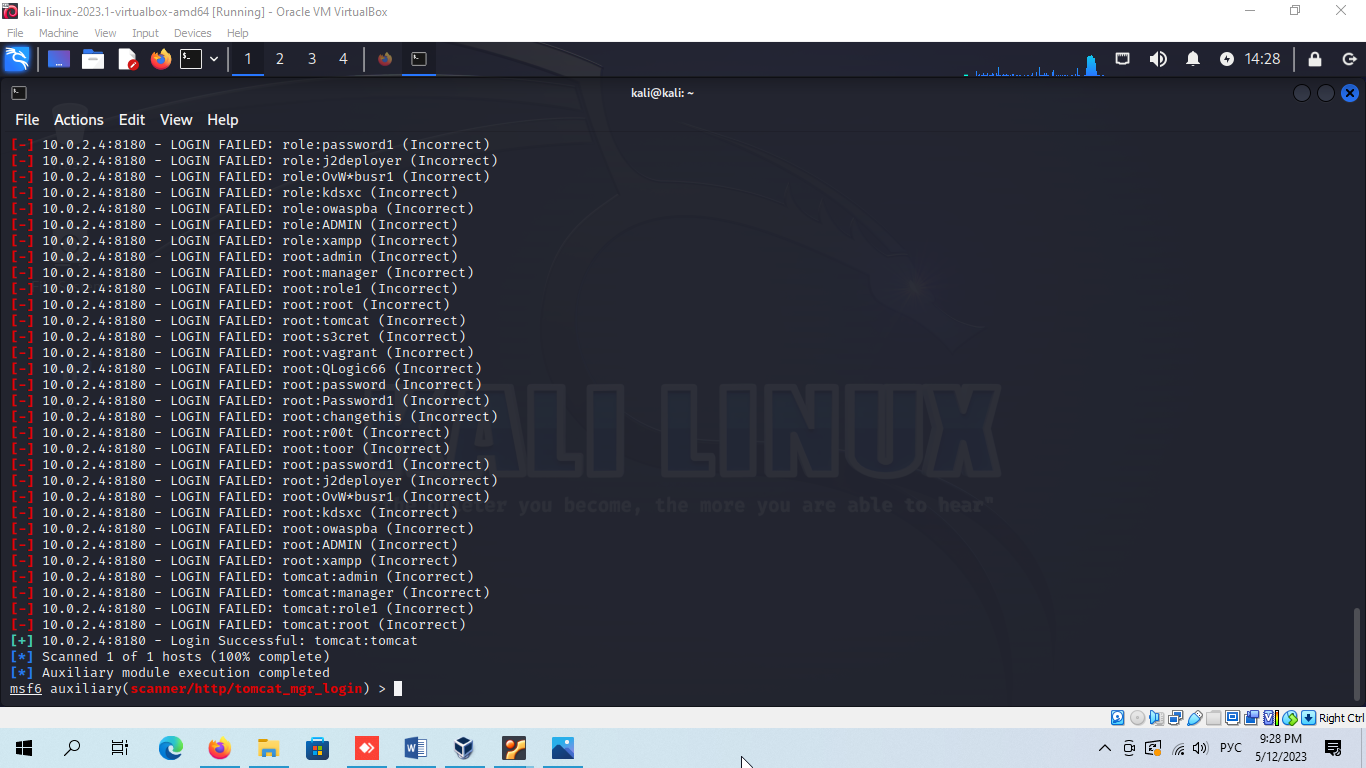
\includegraphics[width=0.85\textwidth]{04_0059}
    \label{img:59}
    \caption{Результат атаки}
  \end{figure}

  В результате атаки также были успешно подобраны логин и пароль - атака успешна.

  \subsection{Эксплуатация готовой атаки}

  Воспользуемся готовым эксплойтом для осуществления атаки на \textit{vsftpd}, посмотрим,
  какие доступны:

  \begin{figure}[H]
    \centering
    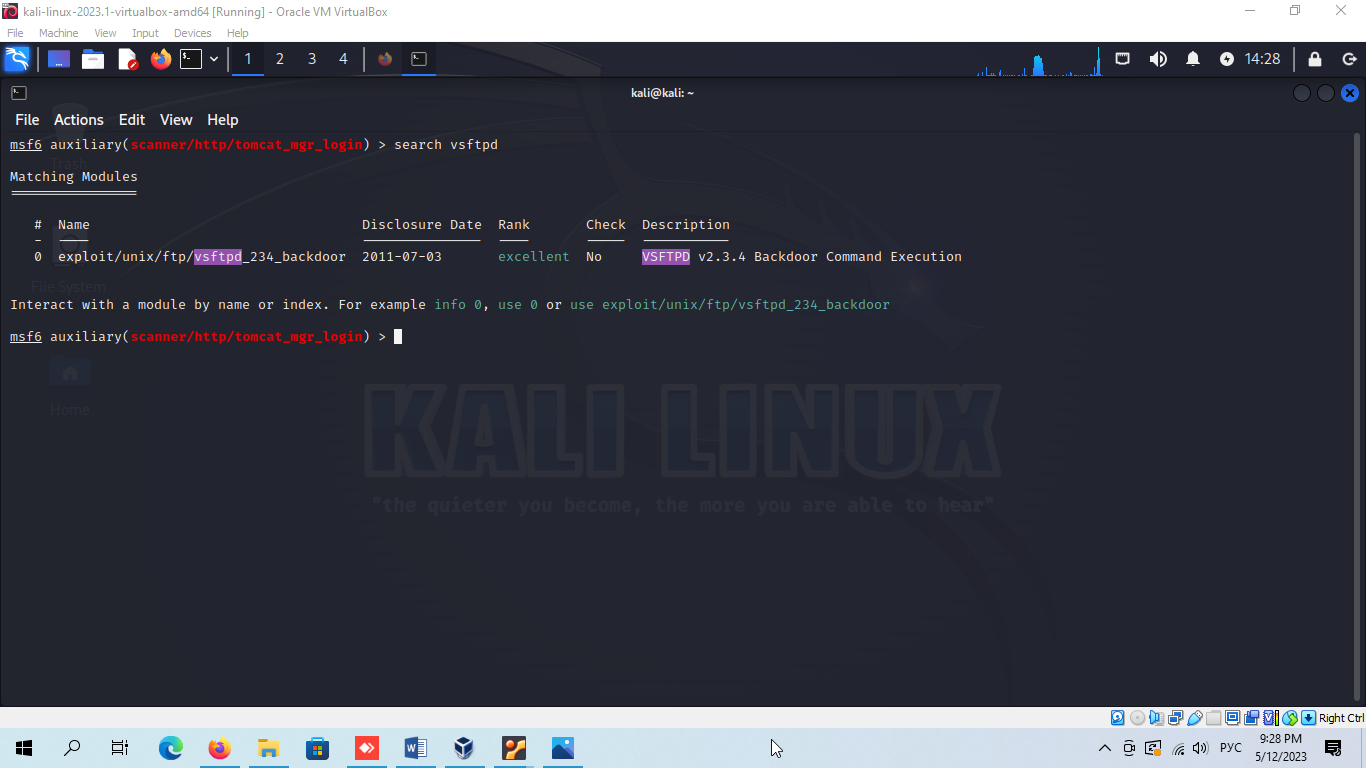
\includegraphics[width=0.85\textwidth]{04_0060}
    \label{img:60}
    \caption{Список эксплойтов для \textit{vsftpd}}
  \end{figure}

  \begin{figure}[H]
    \centering
    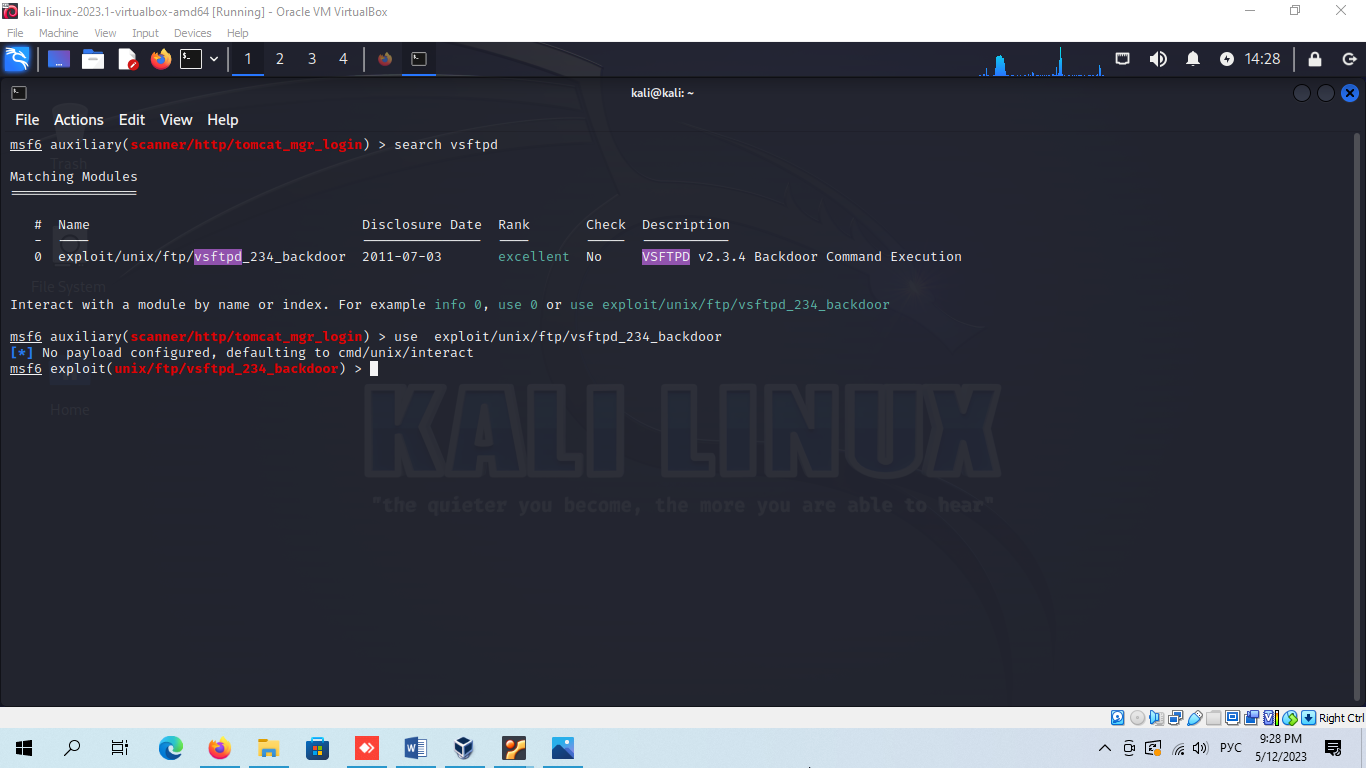
\includegraphics[width=0.85\textwidth]{04_0061}
    \label{img:61}
    \caption{Воспользуемся единственным доступным}
  \end{figure}

  Данный эксплойт требует какую-то нагрузку, посмотрим, что уже встроено в систему:

  \begin{figure}[H]
    \centering
    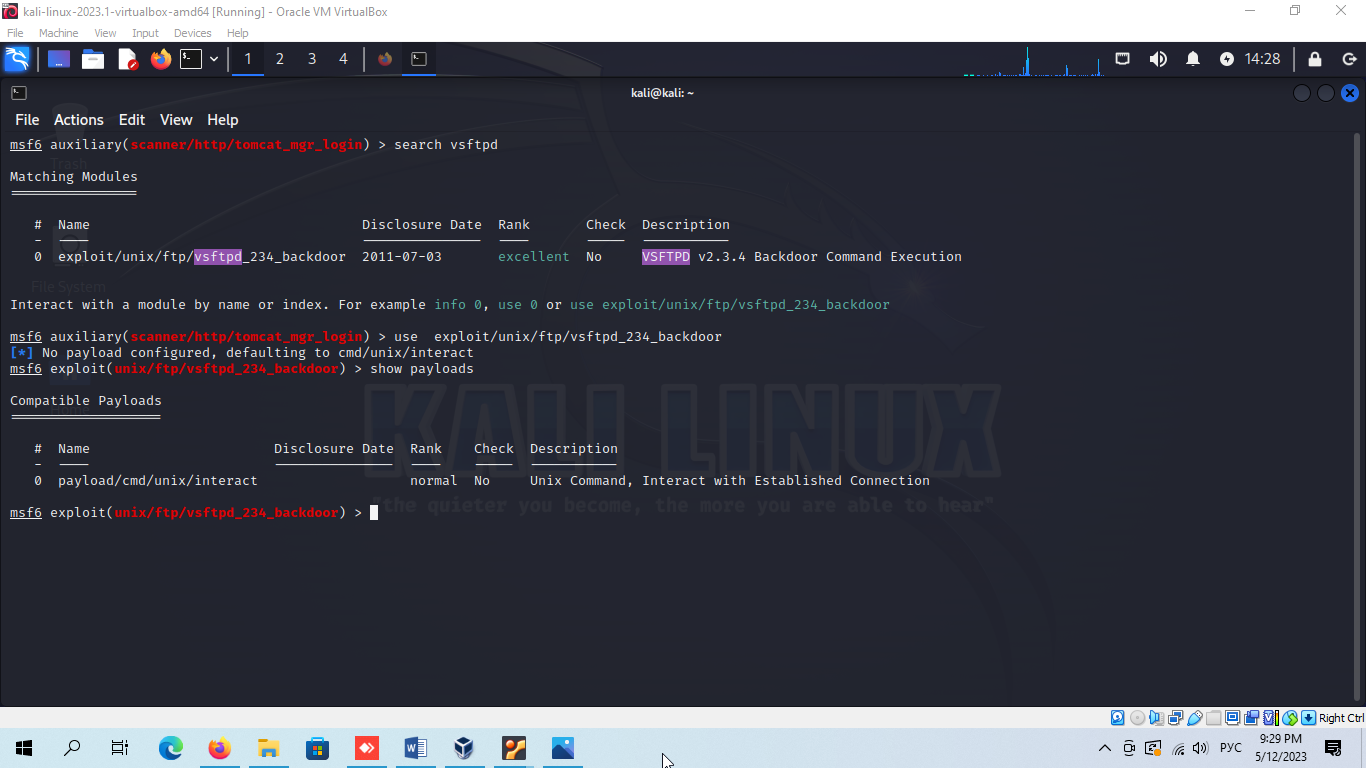
\includegraphics[width=0.85\textwidth]{04_0062}
    \label{img:62}
    \caption{Список доступных нагрузок}
  \end{figure}

  \begin{figure}[H]
    \centering
    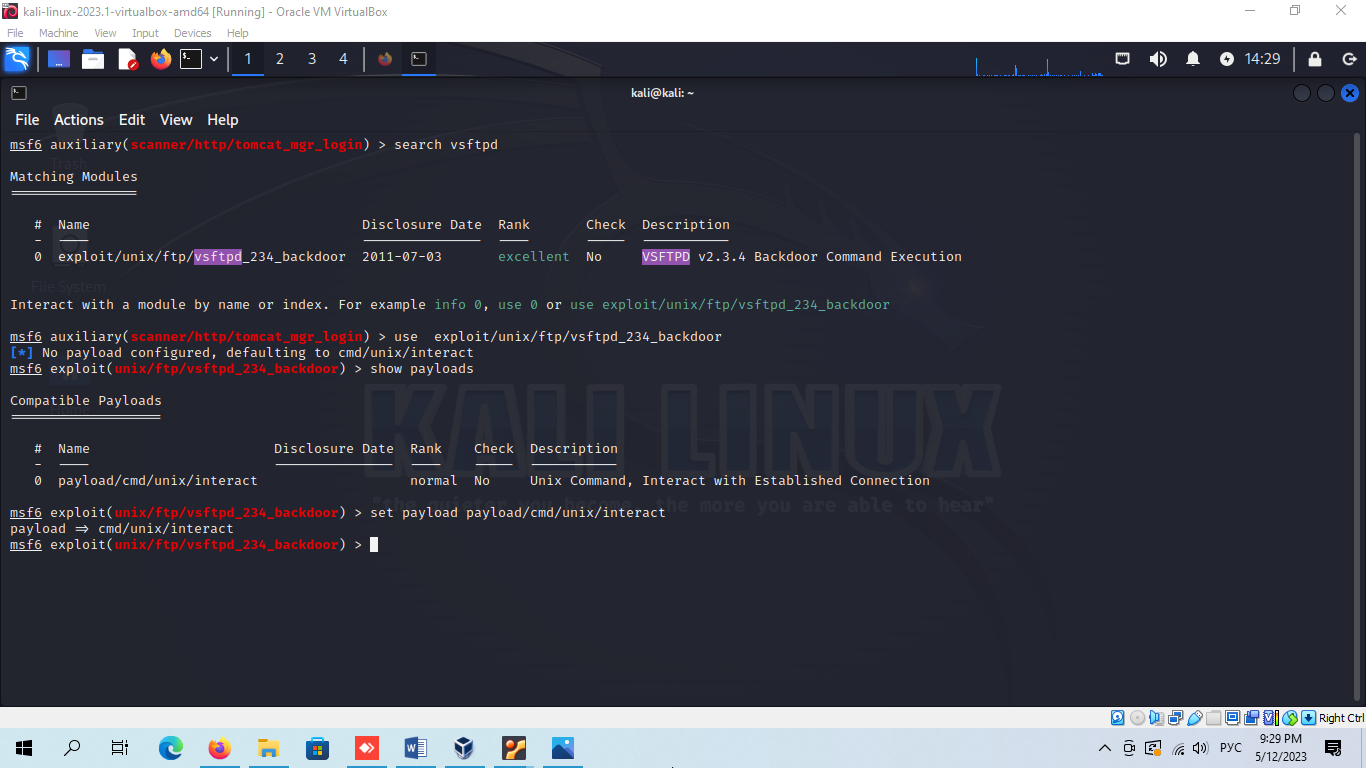
\includegraphics[width=0.85\textwidth]{04_0063}
    \label{img:63}
    \caption{Указываем необходимую - единственную}
  \end{figure}

  Данная нагрузка позволит получить интерактивный \textit{shell} доступ к атакуемой машине.

  \begin{figure}[H]
    \centering
    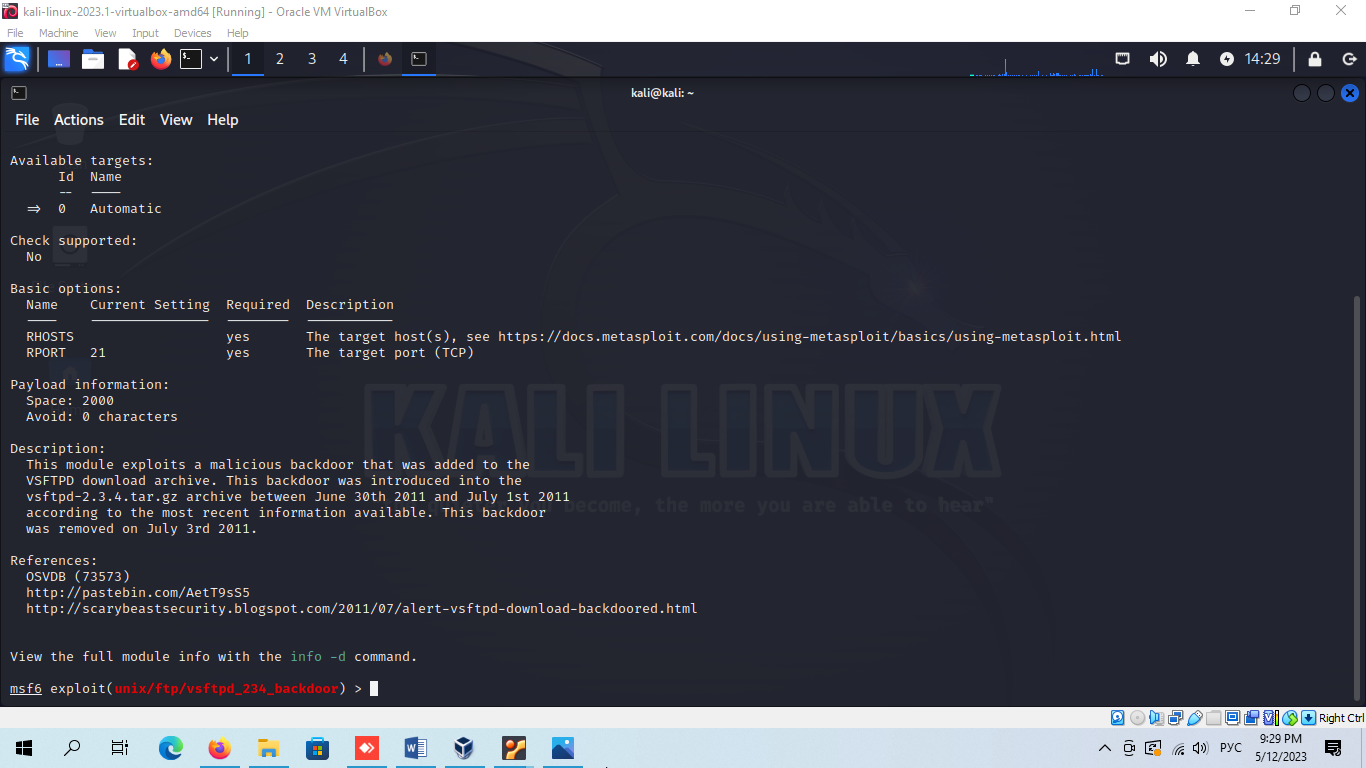
\includegraphics[width=0.85\textwidth]{04_0064}
    \label{img:64}
    \caption{Посмотрим параметры данной атаки}
  \end{figure}

  \begin{figure}[H]
    \centering
    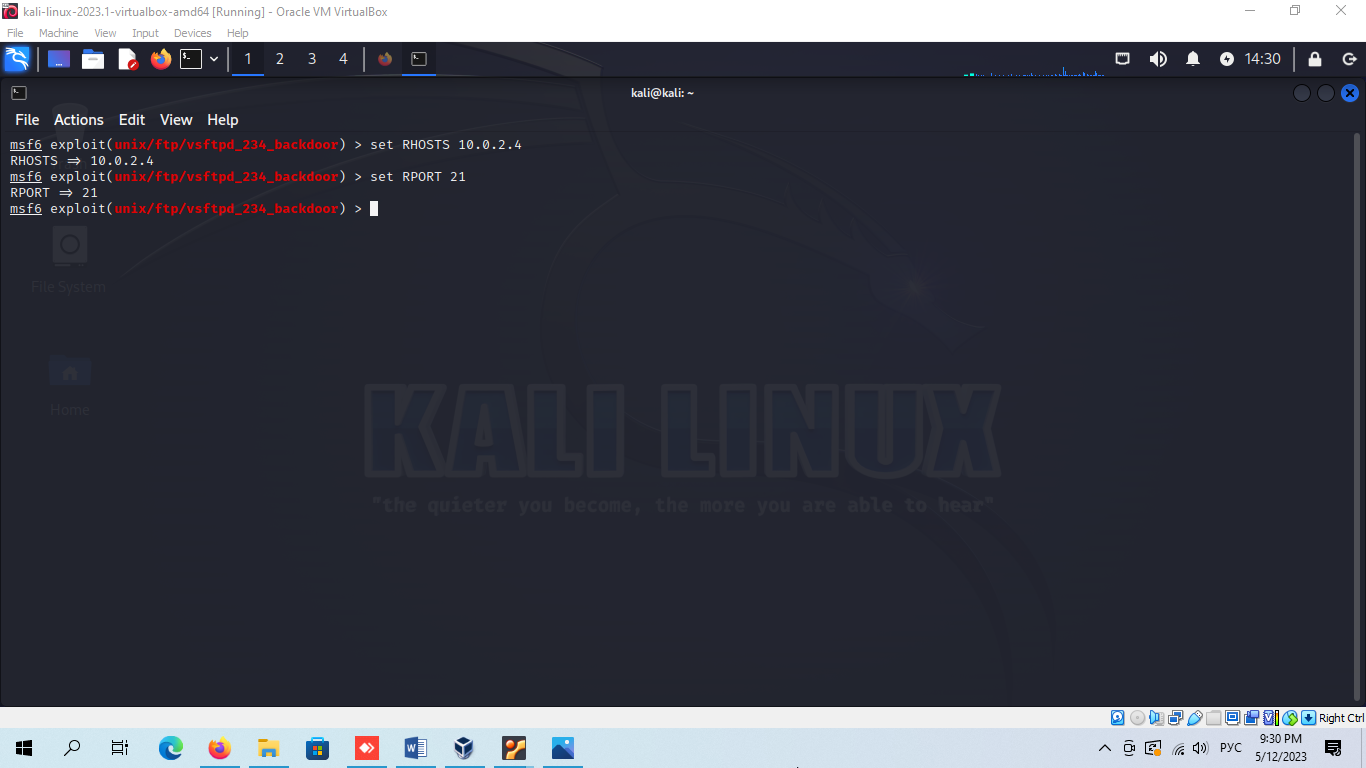
\includegraphics[width=0.85\textwidth]{04_0067}
    \label{img:66}
    \caption{Укажем адрес атакуемой машины и порт атаки}
  \end{figure}

  \begin{figure}[H]
    \centering
    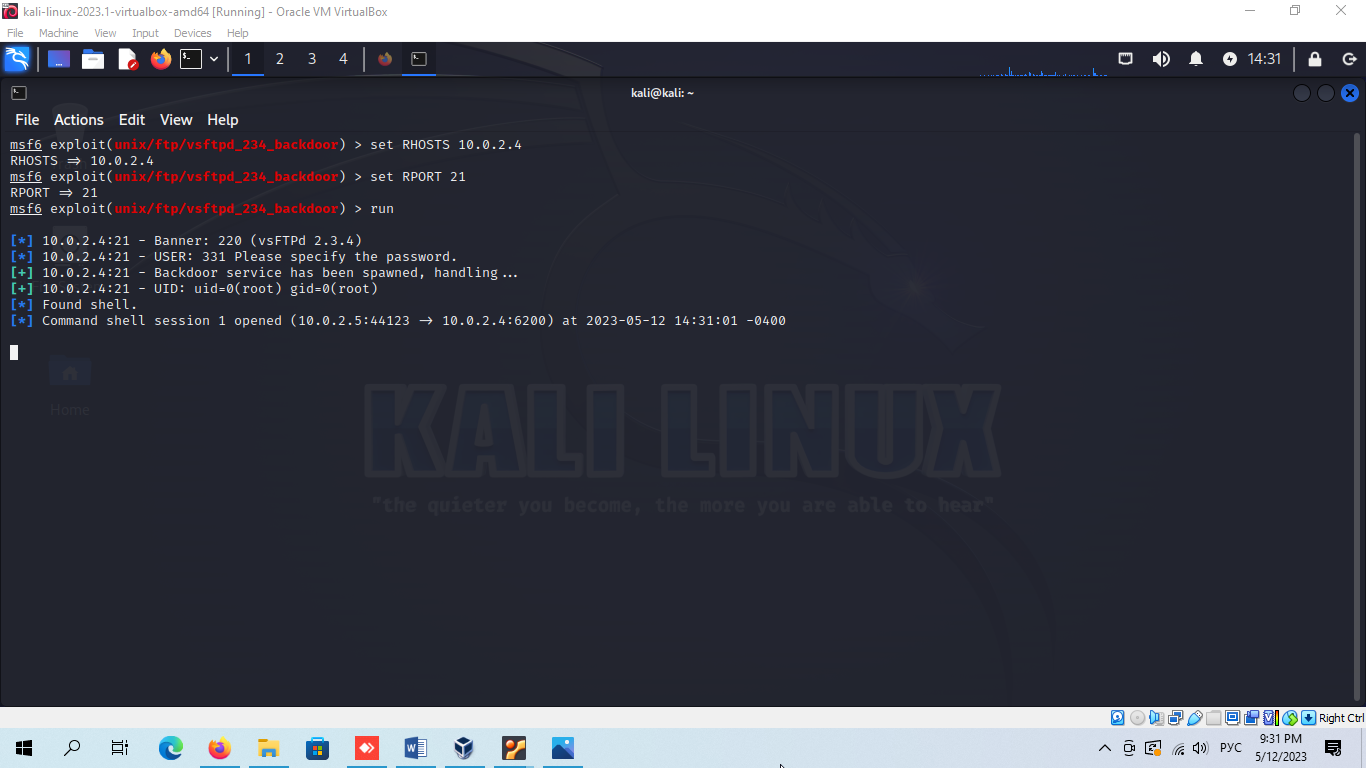
\includegraphics[width=0.85\textwidth]{04_0068}
    \label{img:67}
    \caption{Атака запущена}
  \end{figure}

  \begin{figure}[H]
    \centering
    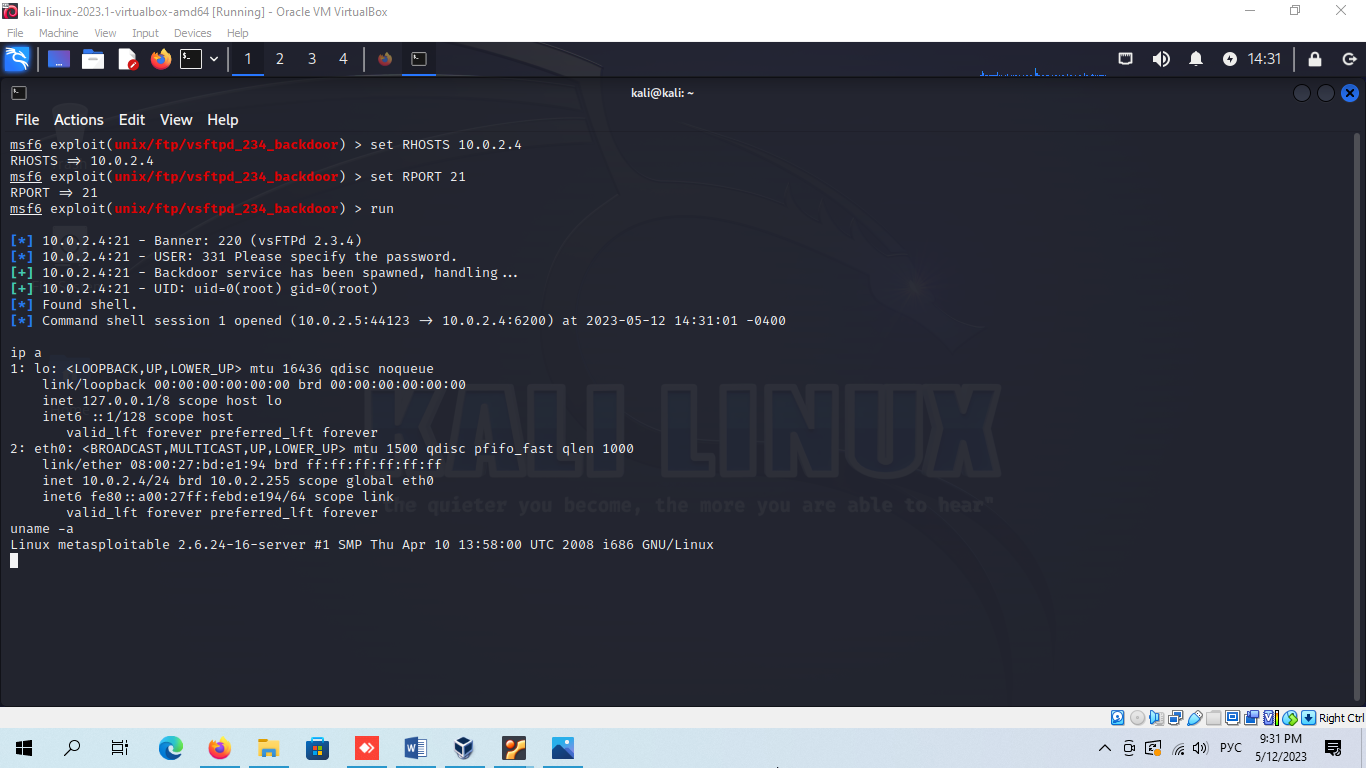
\includegraphics[width=0.85\textwidth]{04_0070}
    \label{img:69}
    \caption{Доступ к атакуемой машине есть}
  \end{figure}

  Попробуем провести похожую атаку на \textit{unrealircd}:

  \begin{figure}[H]
    \centering
    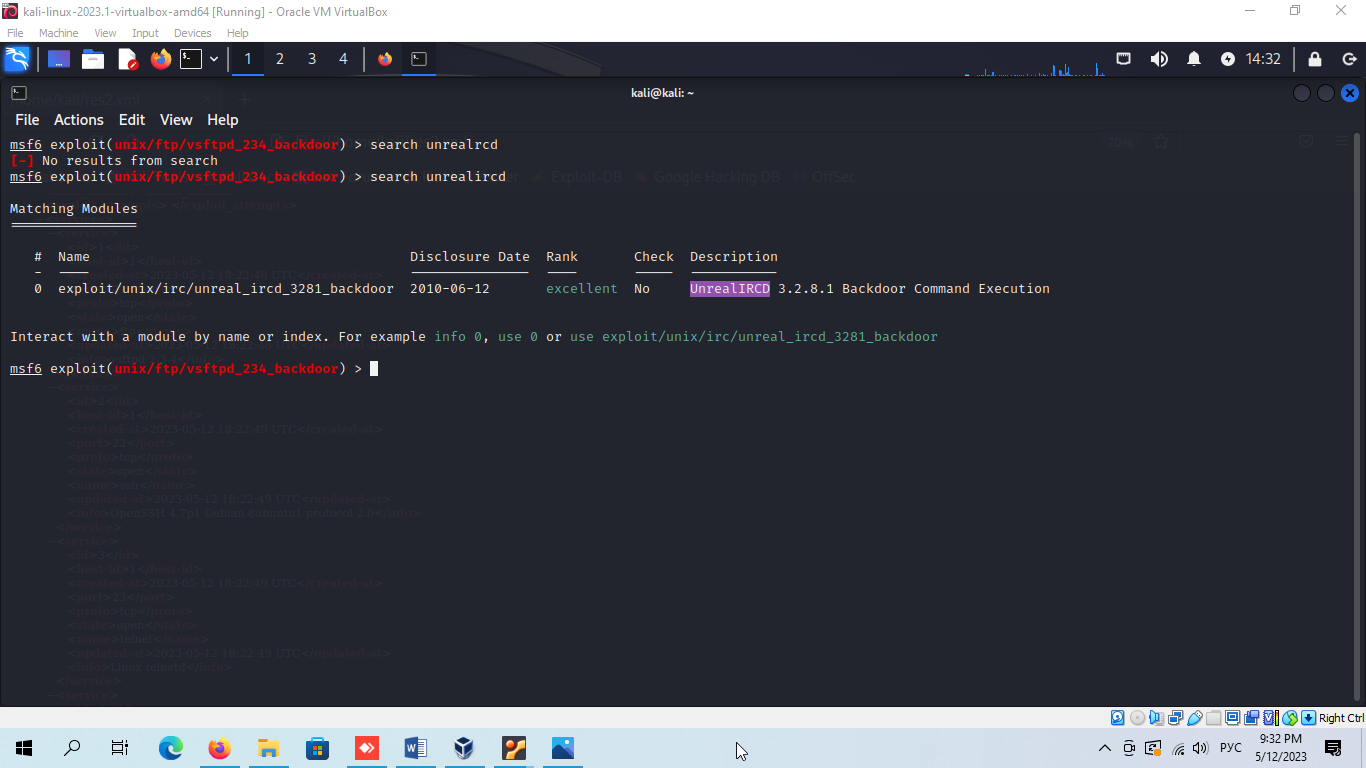
\includegraphics[width=0.85\textwidth]{04_0071}
    \label{img:70}
    \caption{Получим список доступных атак}
  \end{figure}

  \begin{figure}[H]
    \centering
    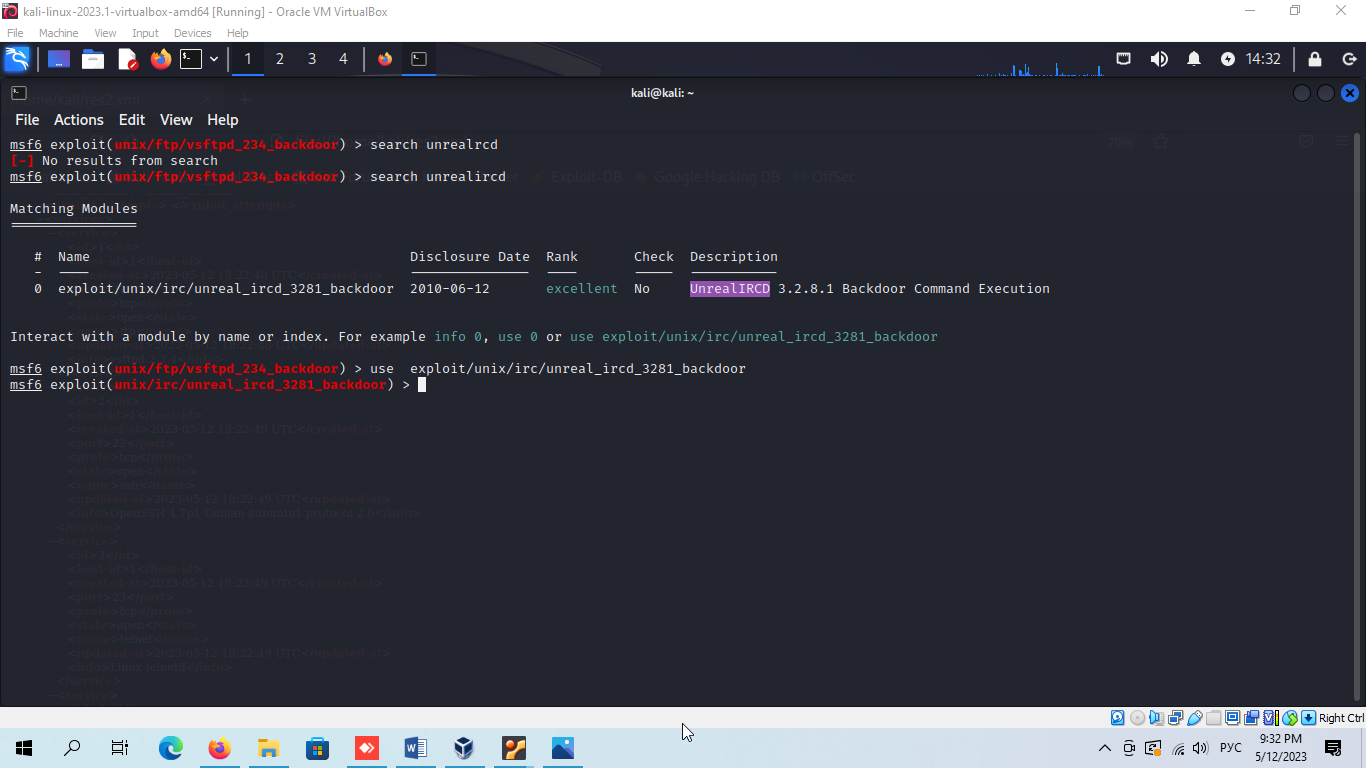
\includegraphics[width=0.85\textwidth]{04_0072}
    \label{img:71}
    \caption{Используем подходящую}
  \end{figure}

  \begin{figure}[H]
    \centering
    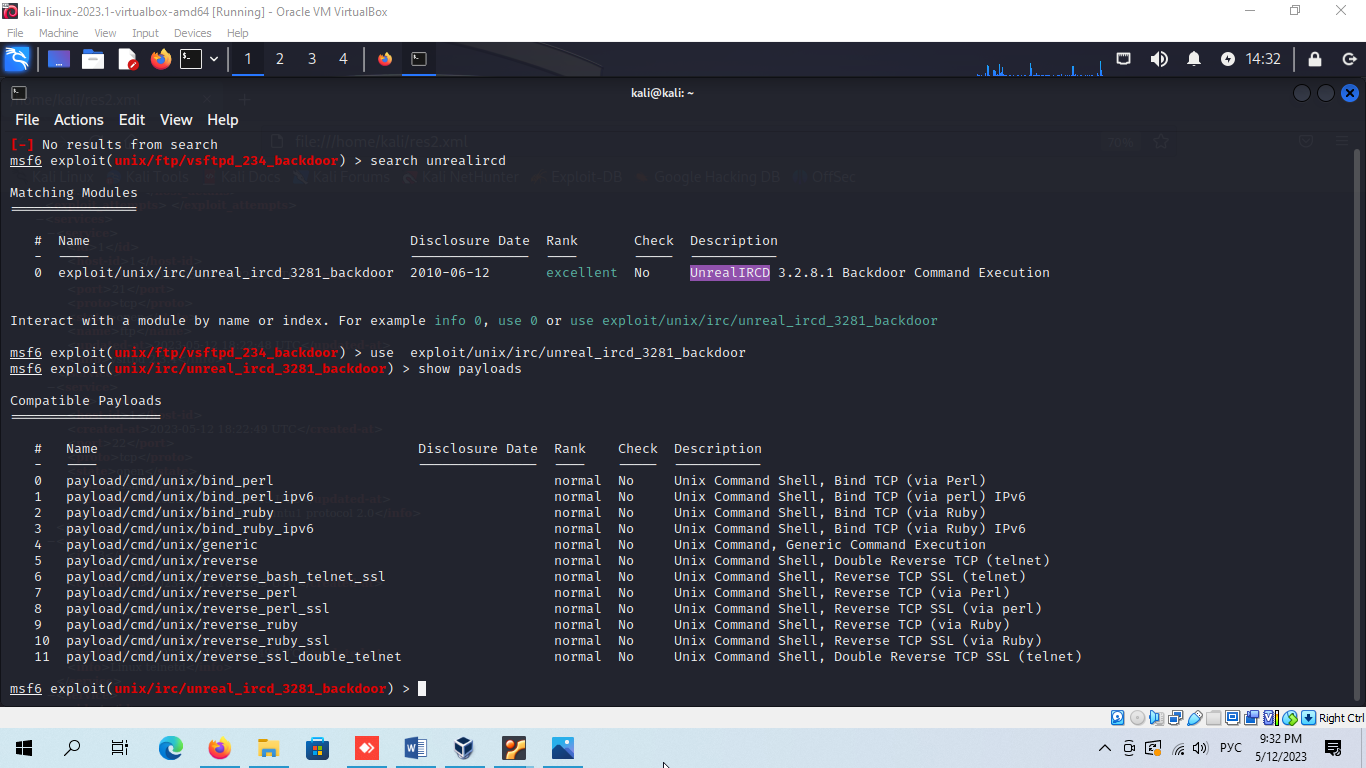
\includegraphics[width=0.85\textwidth]{04_0073}
    \label{img:72}
    \caption{Смотрим, какие есть нагрузки для атаки}
  \end{figure}

  \begin{figure}[H]
    \centering
    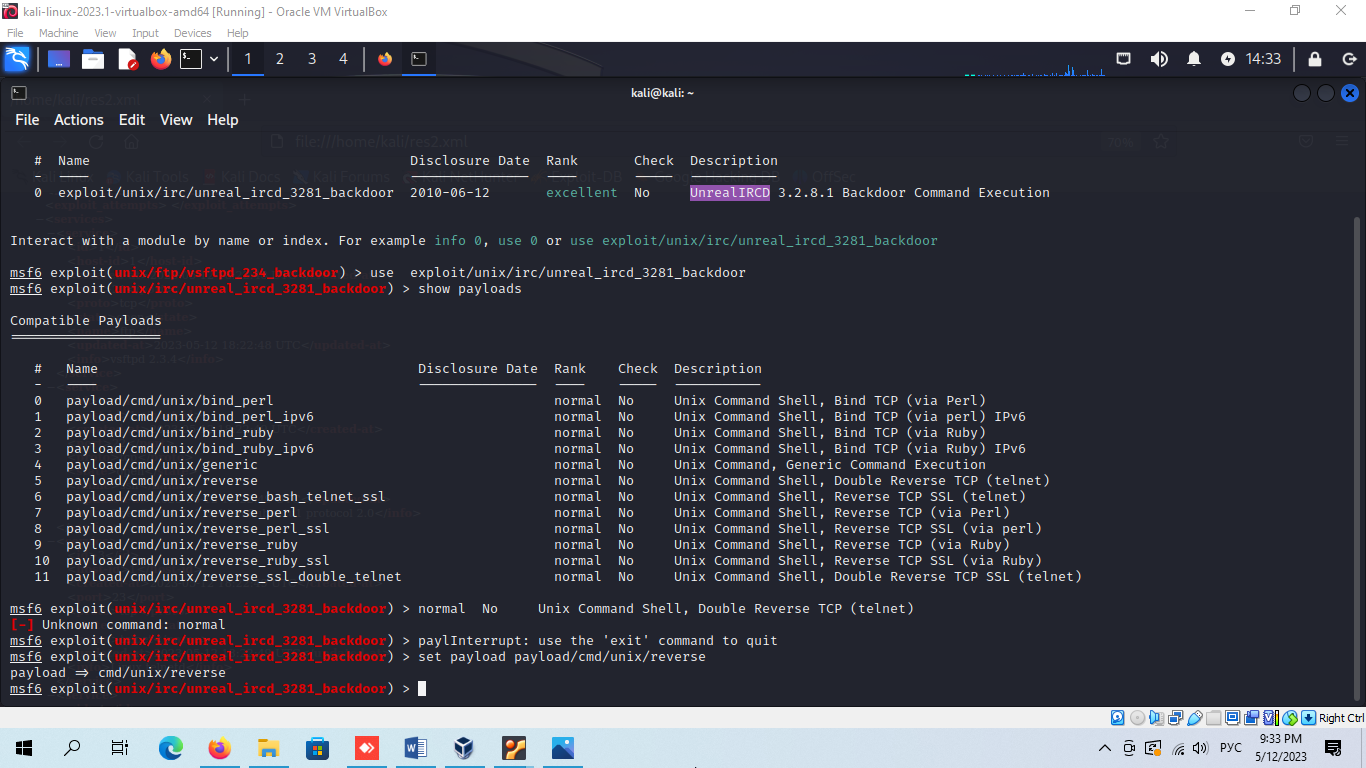
\includegraphics[width=0.85\textwidth]{04_0074}
    \label{img:73}
    \caption{Указываем подходящую}
  \end{figure}

  Данная нагрузка позволит получить такой же интерактивный \textit{shell} доступ к атакуемой машине.

  \begin{figure}[H]
    \centering
    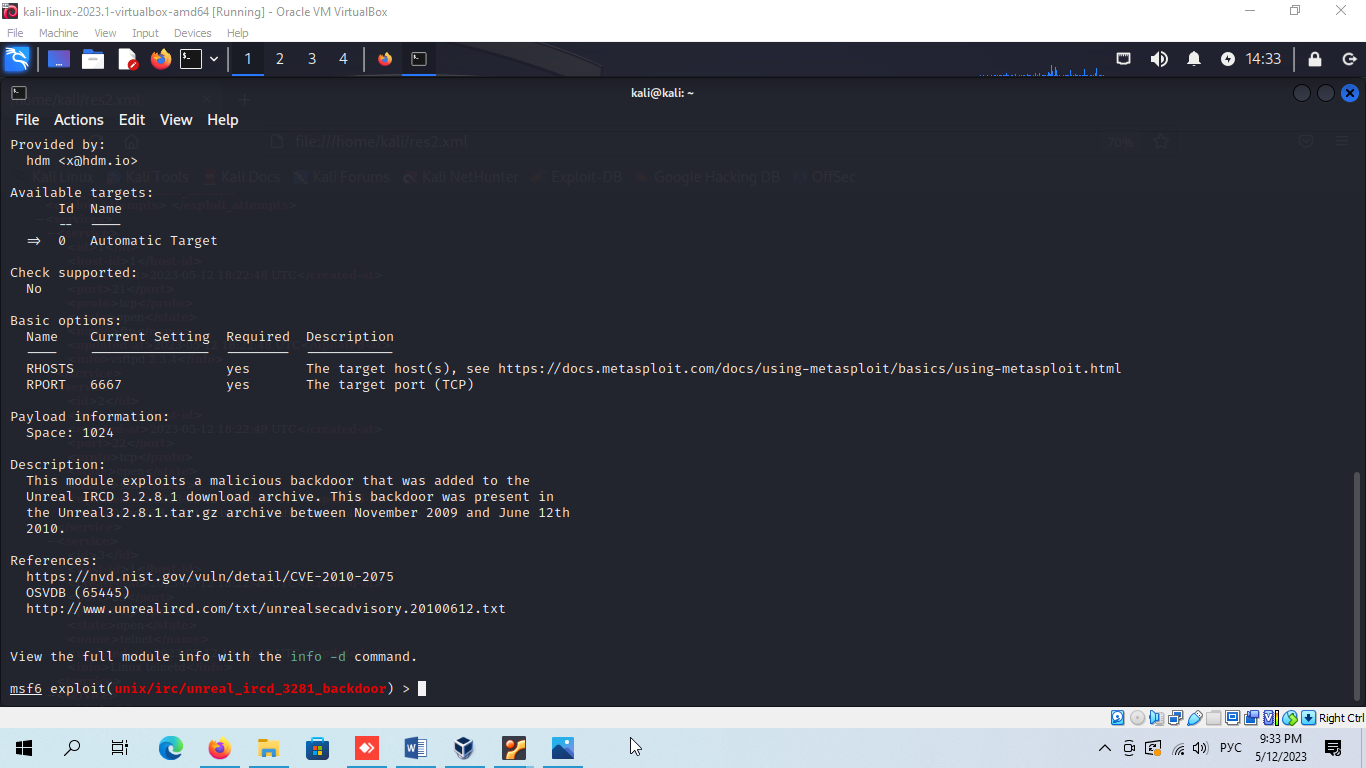
\includegraphics[width=0.85\textwidth]{04_0075}
    \label{img:74}
    \caption{Смотрим список доступных для настройки параметров}
  \end{figure}

  \begin{figure}[H]
    \centering
    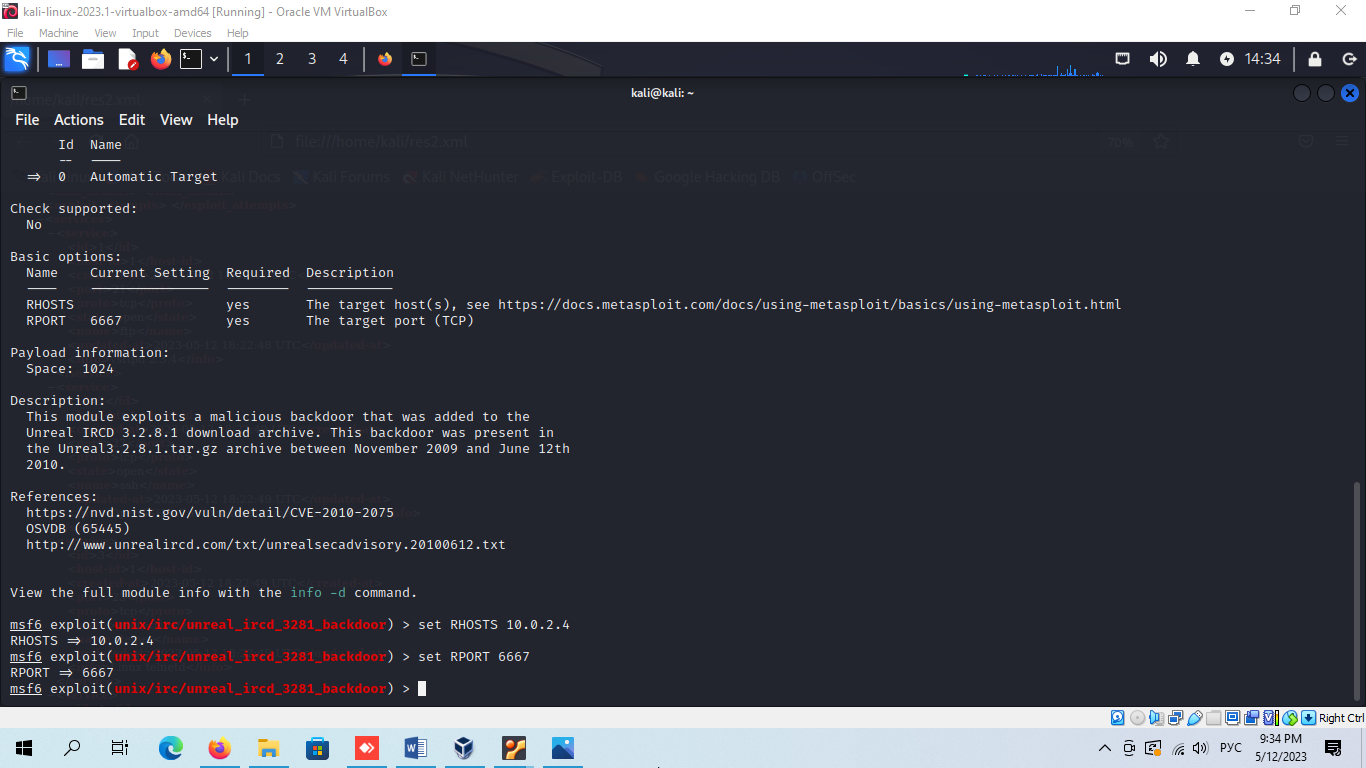
\includegraphics[width=0.85\textwidth]{04_0076}
    \label{img:75}
    \caption{Указываем необходимые параметры}
  \end{figure}

  Здесь также потребовалось указать \textit{LHOST} - адрес атакующей машины (
    необходимо для выбранной полезной нагрузки
  ).

  \begin{figure}[H]
    \centering
    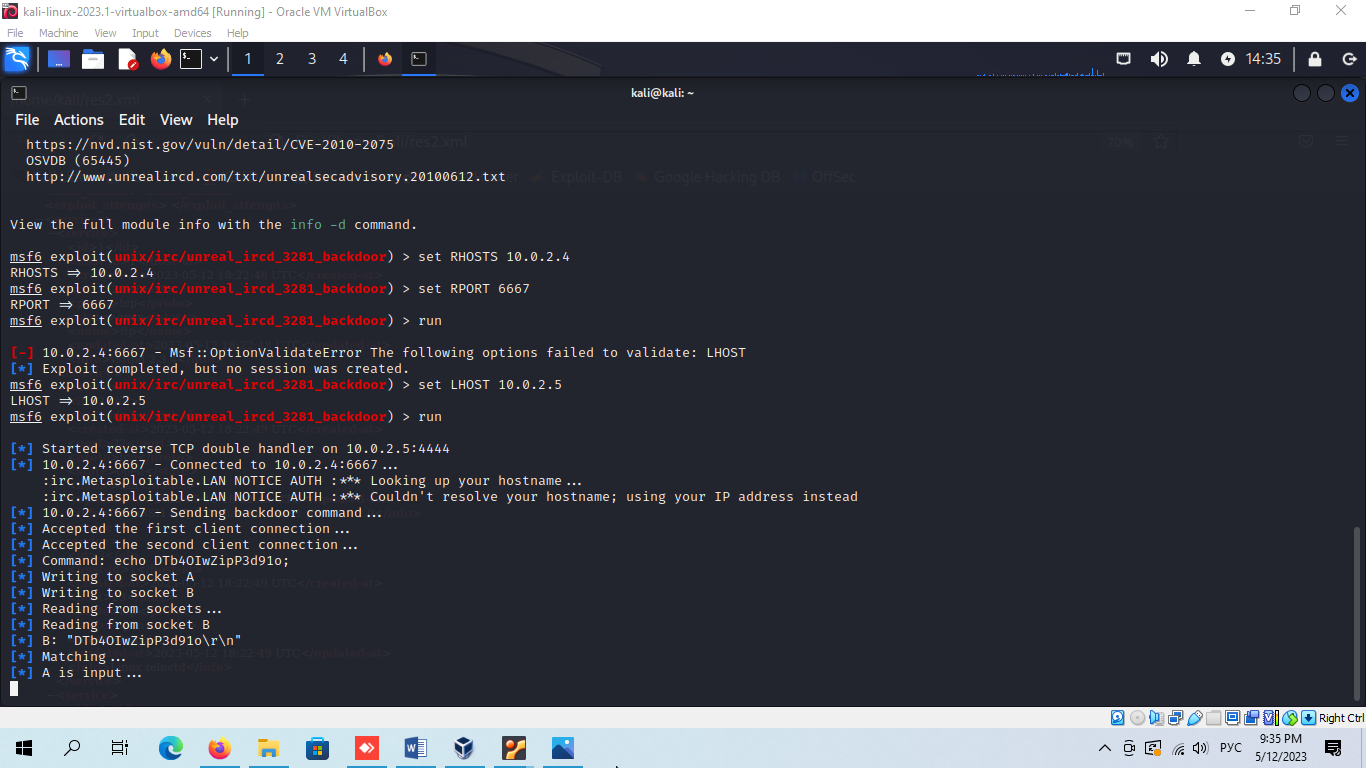
\includegraphics[width=0.85\textwidth]{04_0077}
    \label{img:76}
    \caption{Запускаем атаку}
  \end{figure}

  \begin{figure}[H]
    \centering
    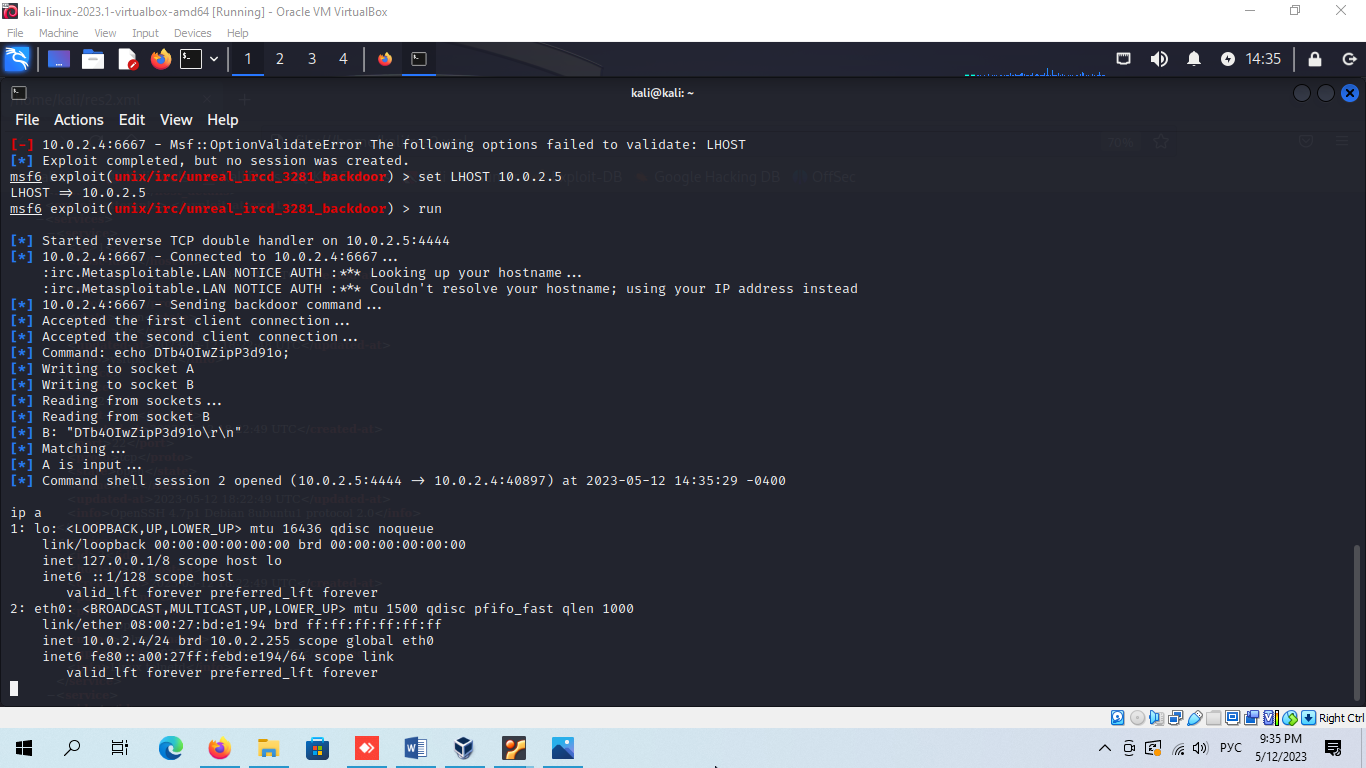
\includegraphics[width=0.85\textwidth]{04_0078}
    \label{img:78}
    \caption{Доступ к атаукемой машине}
  \end{figure}

  Атака произведена успешно.

  \subsection{Самостоятельная атака}

  Изучив результаты сканирования можно увидеть, что на атакуемой машине запущено
  достаточно большое количество сервисов, посмотрим, какие атаки на данные сервисы
  есть в базе \textit{MSF}:

  \begin{figure}[H]
    \centering
    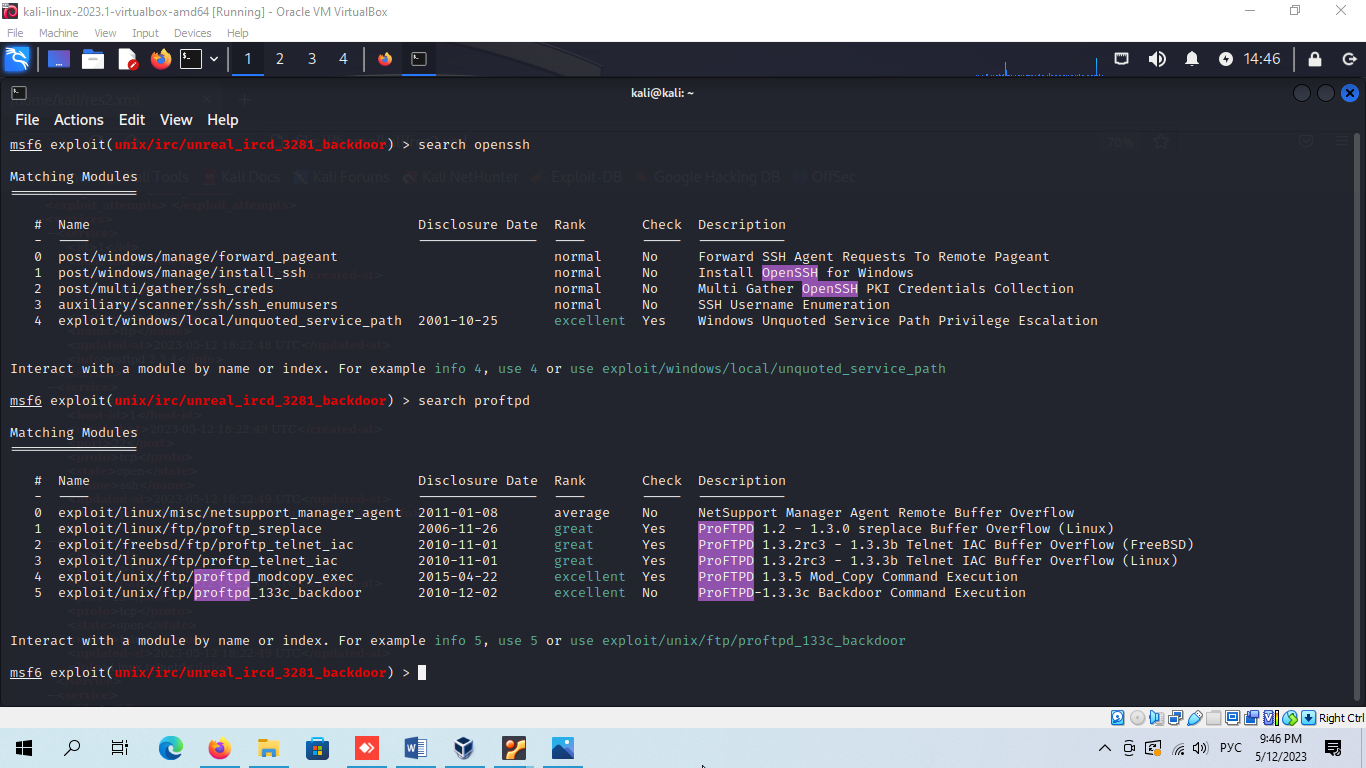
\includegraphics[width=0.85\textwidth]{04_0080}
    \label{img:79}
    \caption{Проверяю уязвимости для найденных сервисов}
  \end{figure}

  Подхоядщих атак на \textit{OpenSSH} не нашлось, а атаки, найденные
  для \textit{proftpd} работают на версиях демона, отличных от установленного на атакуемой машине.

  \begin{figure}[H]
    \centering
    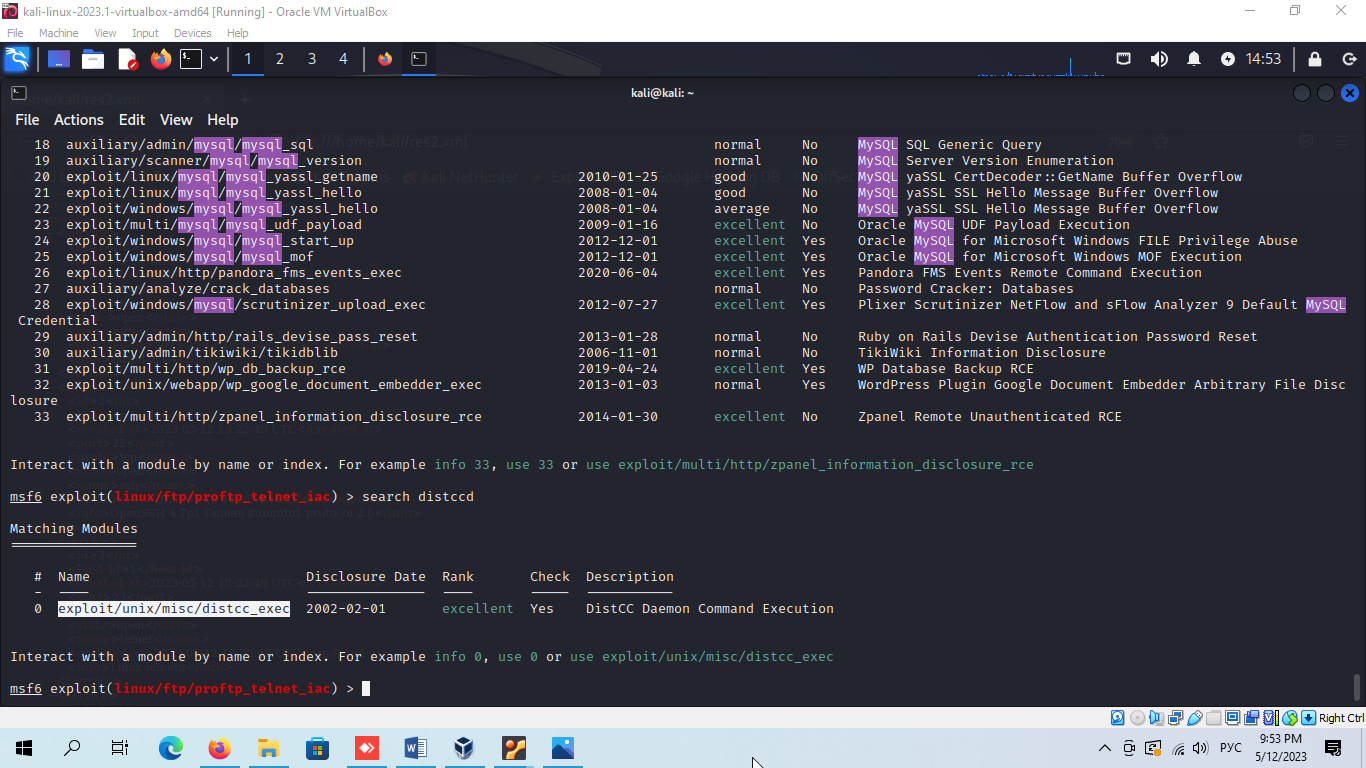
\includegraphics[width=0.85\textwidth]{04_0087}
    \label{img:86}
    \caption{Список атак на \textit{distcc}}
  \end{figure}

  А вот на \textit{distcc} есть подходящая атака - проведем ее.

  \begin{figure}[H]
    \centering
    \includegraphics[width=0.85\textwidth]{04_0088}
    \label{img:87}
    \caption{Посмотрим список доступных полезных нагрузок}
  \end{figure}

  \begin{figure}[H]
    \centering
    \includegraphics[width=0.85\textwidth]{04_0093}
    \label{img:93}
    \caption{Укажем  необходимую нагрузку и параметры атаки}
  \end{figure}

  \begin{figure}[H]
    \centering
    \includegraphics[width=0.85\textwidth]{04_0095}
    \label{img:94}
    \caption{Результат атаки - \textit{shell} доступ к атакуемой машине}
  \end{figure}

  Получен доступ к атакуемой машине - атака проведена успешно.

  \section{Вывод}

  В ходе данной работы мне удалось научиться сканировать машины при помощи
  встроенного в \textit{Metasploit nmap}, проводить различные атаки, как
  использующие простой полный перебор, так и специализированные эксплойти,
  а так же искать подходящую уязвимость исходя из результатов анализа системы.

\end{document}

